\section[Unaligned Membrane Images]{Factoring Out Symmetries in Two--Dimensional~Membrane~Images Using~Angular~Synchronization}


\begin{frame}[label=current]{Ordering of Two-Dimensional Membrane Images}
    We  order the images using the scattering transform + DMAPS\\
    
    \centering
    \begin{tikzpicture}
    	\node[anchor=south west] (image) {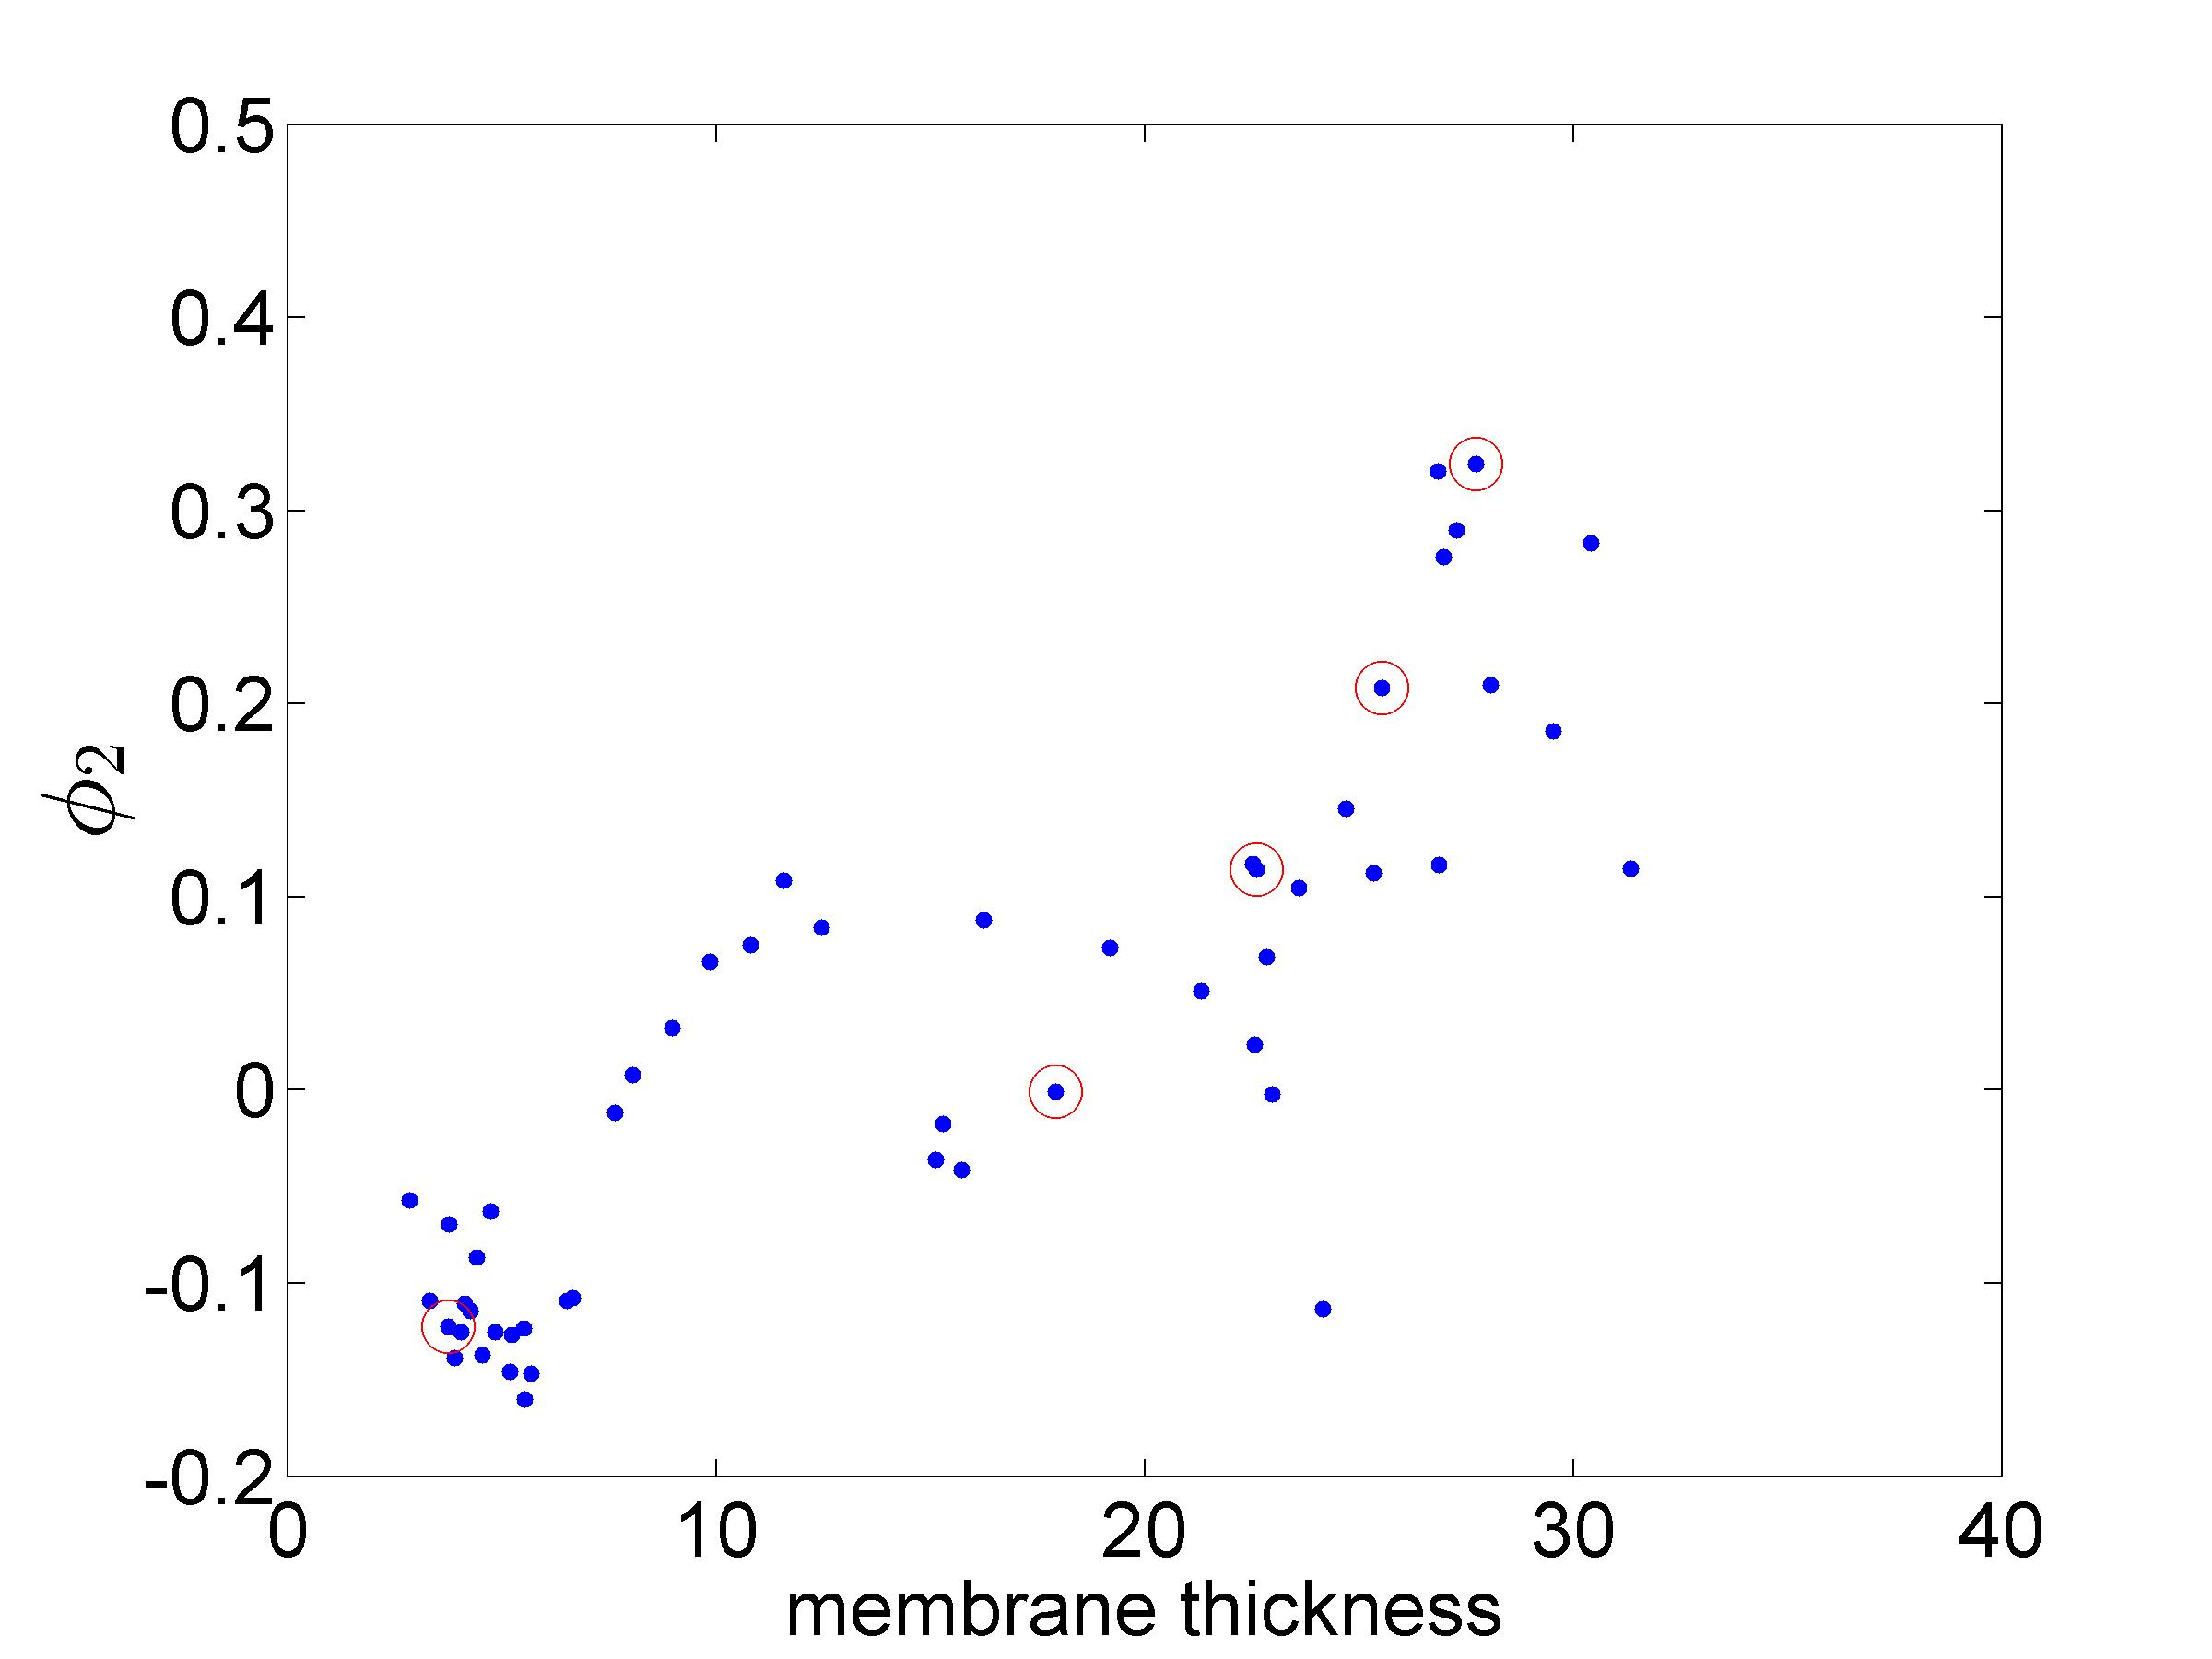
\includegraphics[width=0.4\textwidth]{DMAPS_membrane_scat_time_corr2}};
    	\begin{scope}[x={(image.south east)},y={(image.north west)}]
    	%\draw[help lines,xstep=.05,ystep=.05] (0,0) grid (1,1);
    	\node(x1) at (0.23,0.23) {};
    	\node(x2) at (0.50,0.38) {};
    	\node(x3) at (0.57,0.51) {};
    	\node(x4) at (0.61,0.62) {};
    	\node(x5) at (0.64,0.74) {};
    	\end{scope}
    	\node[below=0.2in of image](fig3) {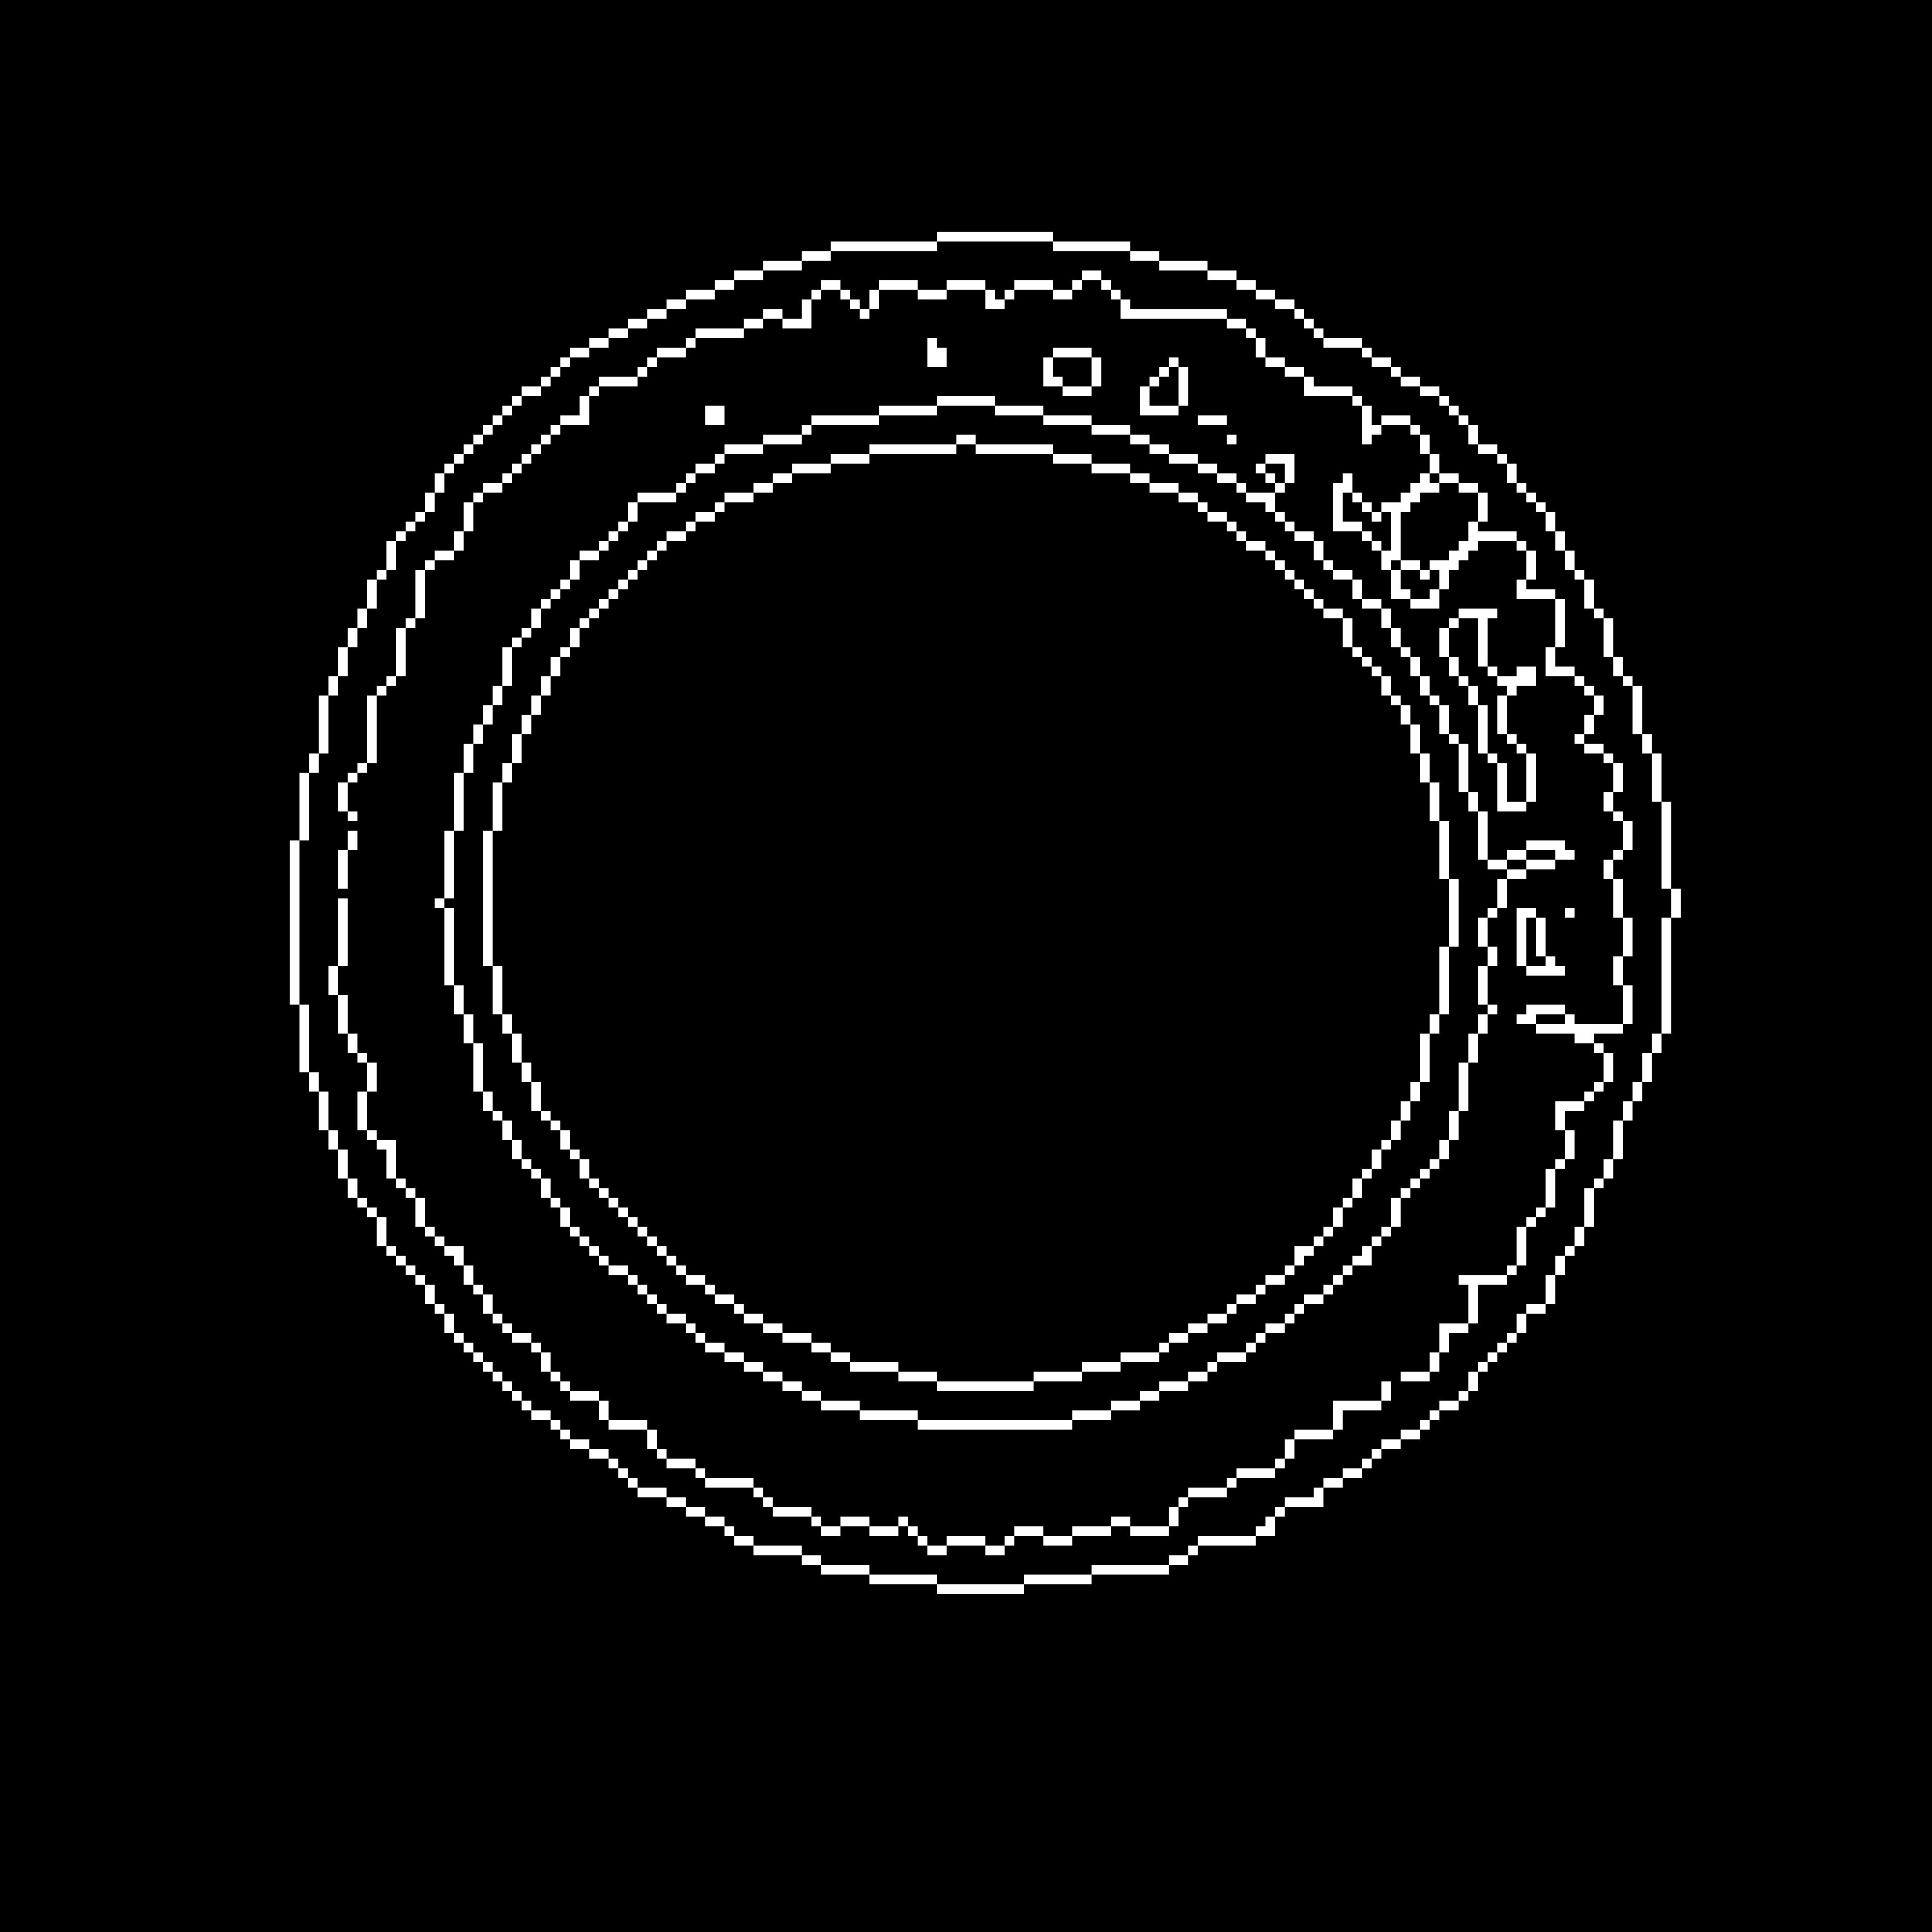
\includegraphics[width=0.1\textwidth]{membrane_scat_3}};		
    	\node[left=0.1in of fig3](fig2) {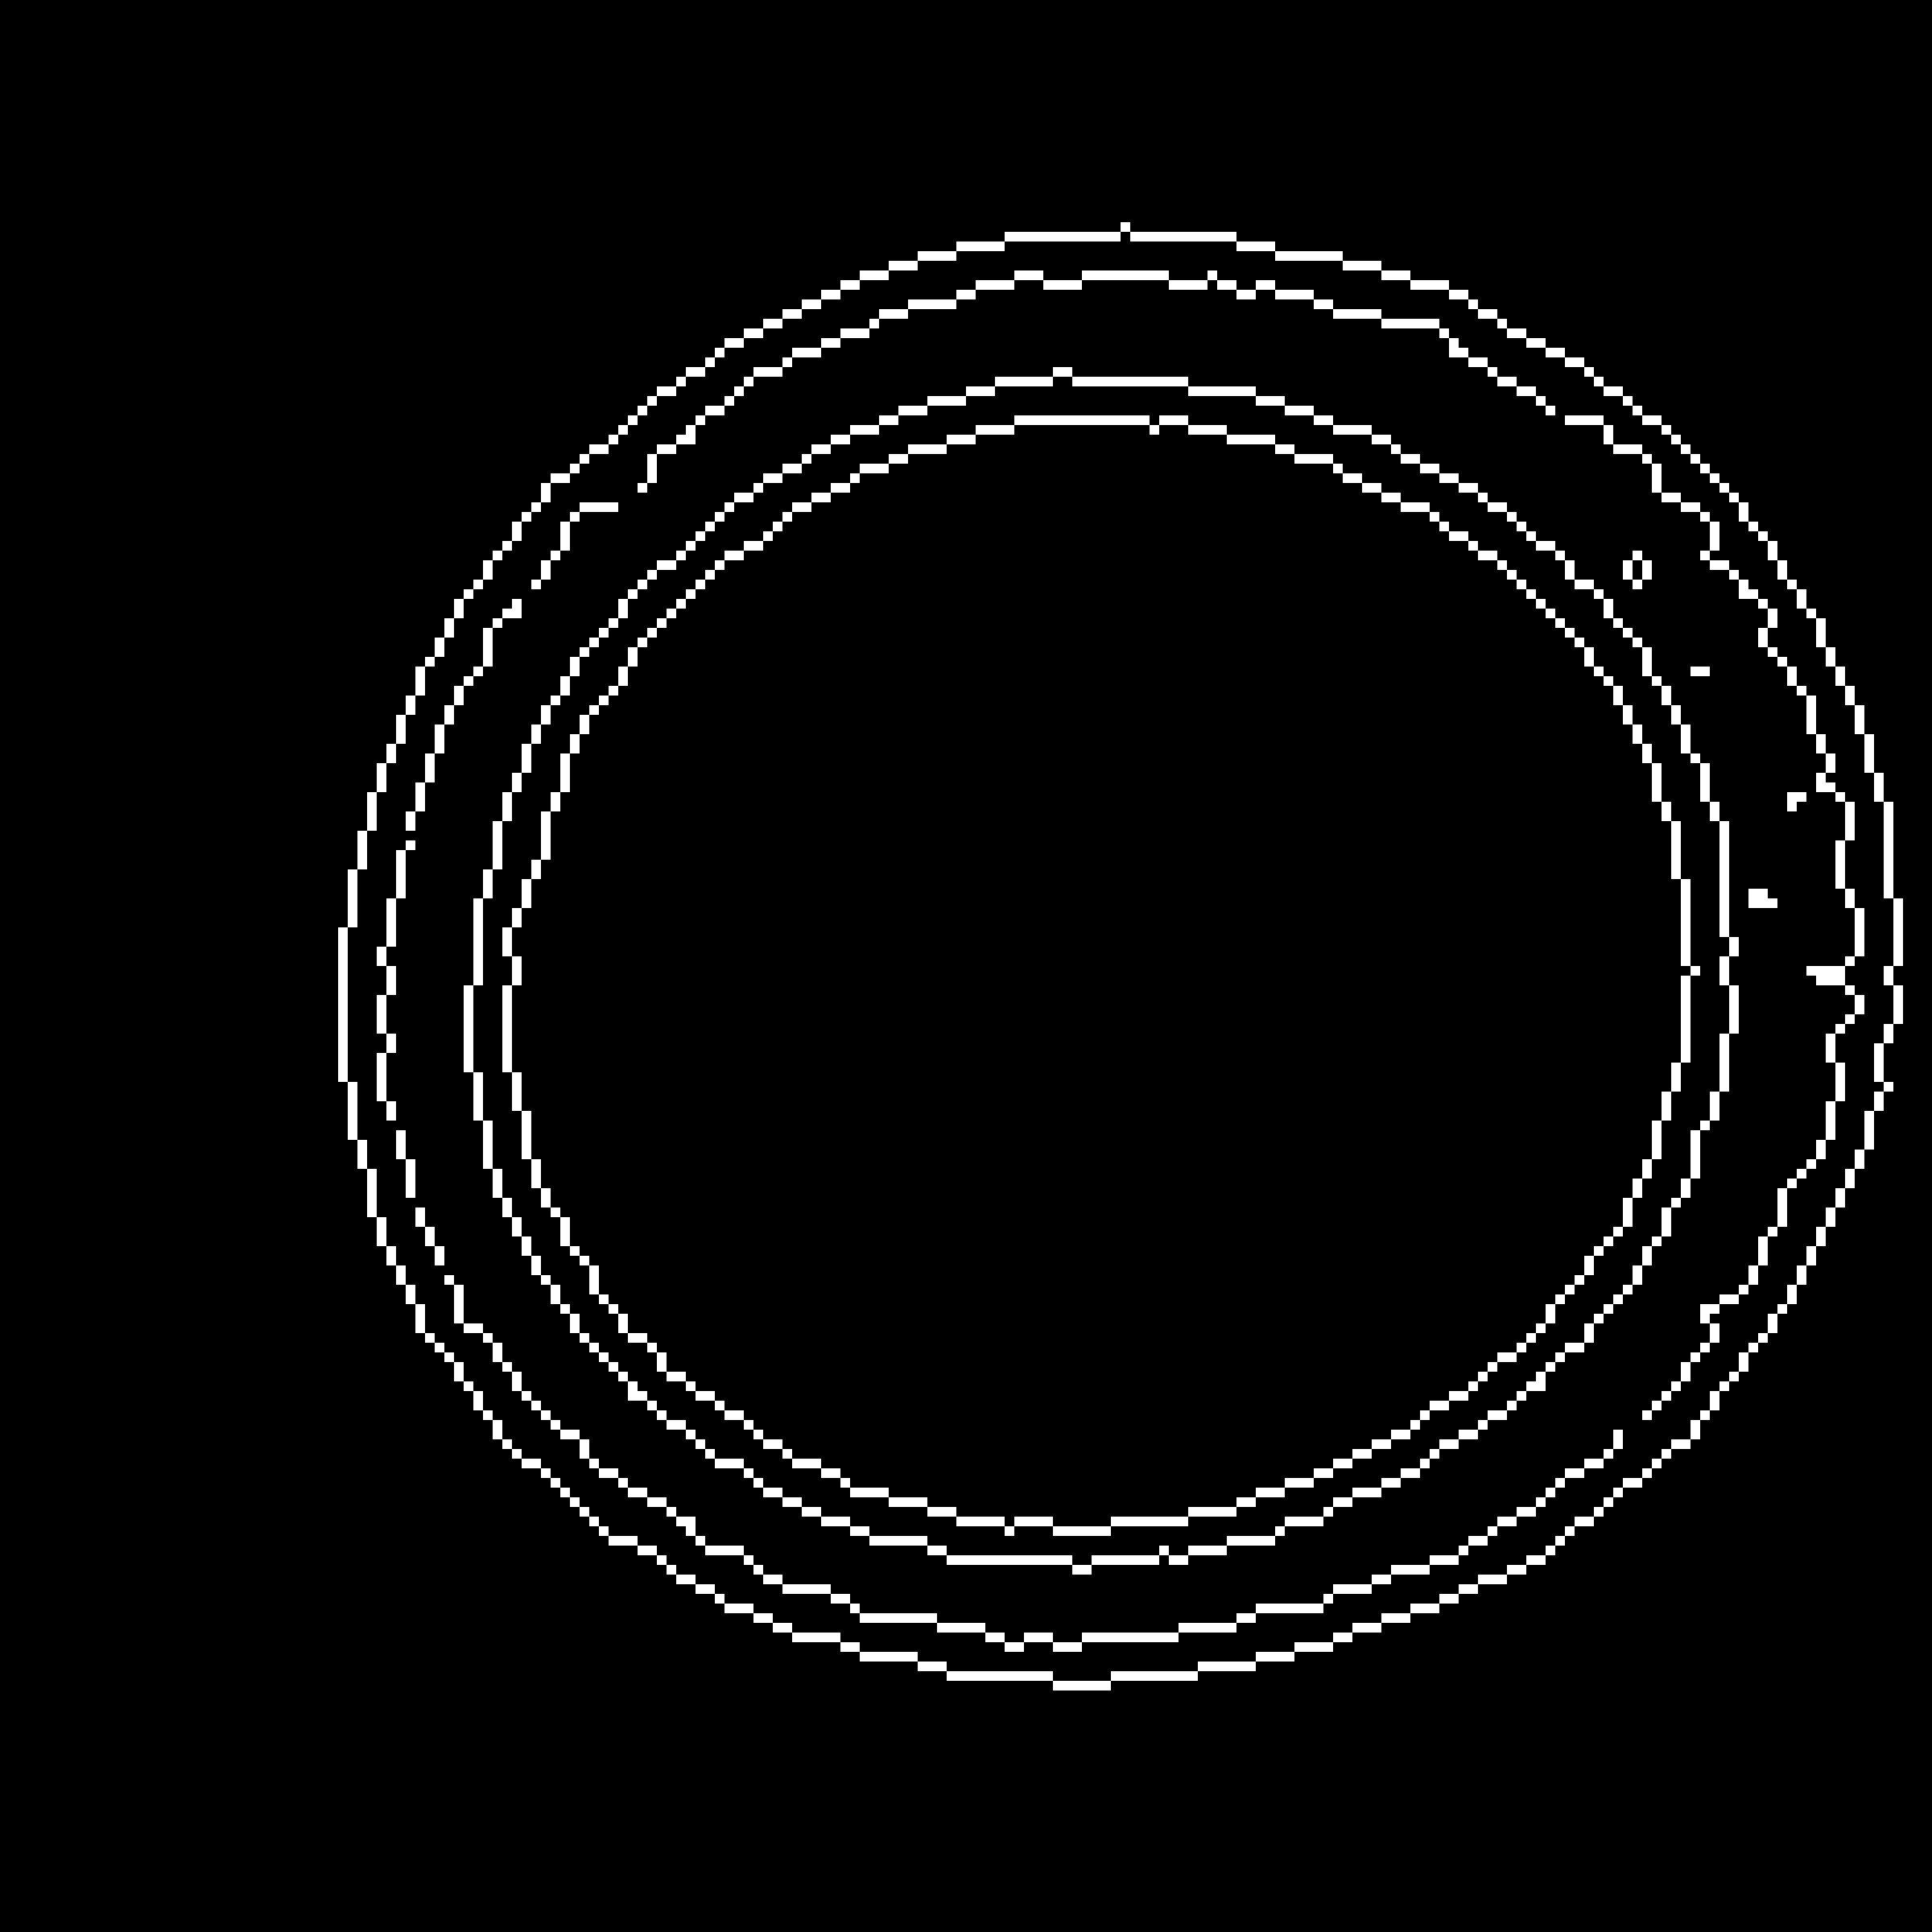
\includegraphics[width=0.1\textwidth]{membrane_scat_2}};
    	\node[left=0.1in of fig2](fig1) {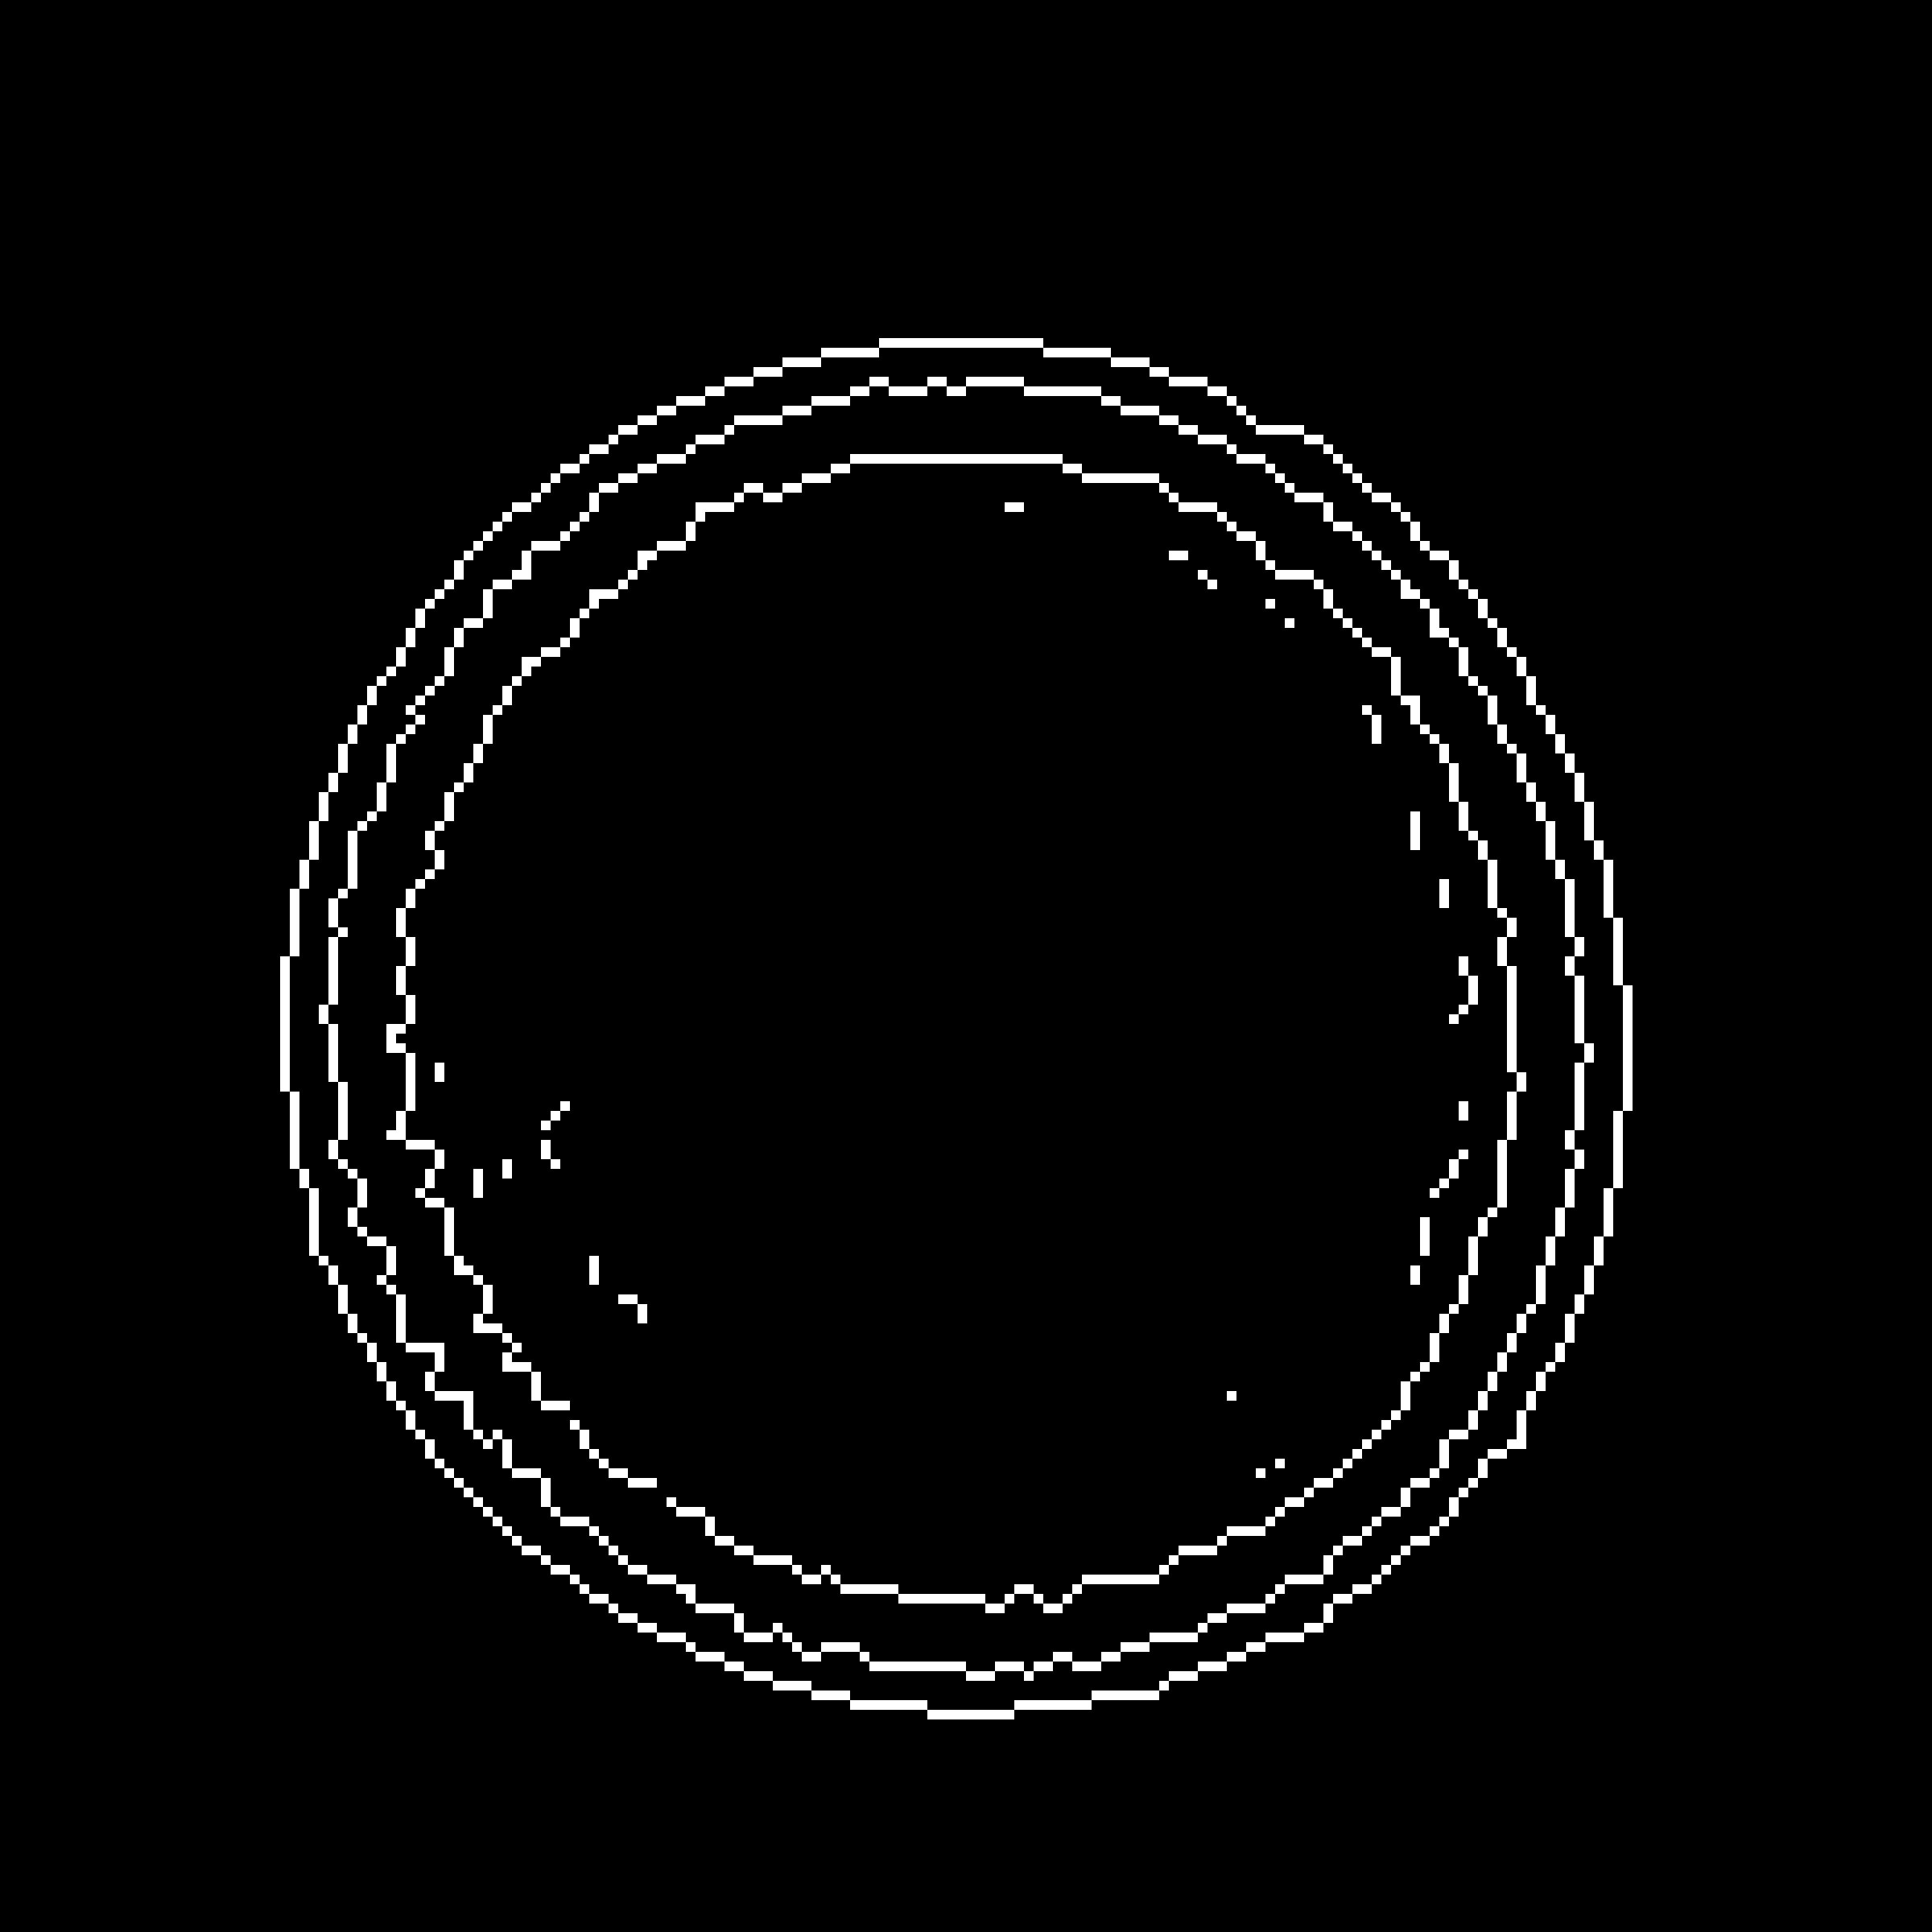
\includegraphics[width=0.1\textwidth]{membrane_scat_1}};	
    	\node[right=0.1in of fig3](fig4) {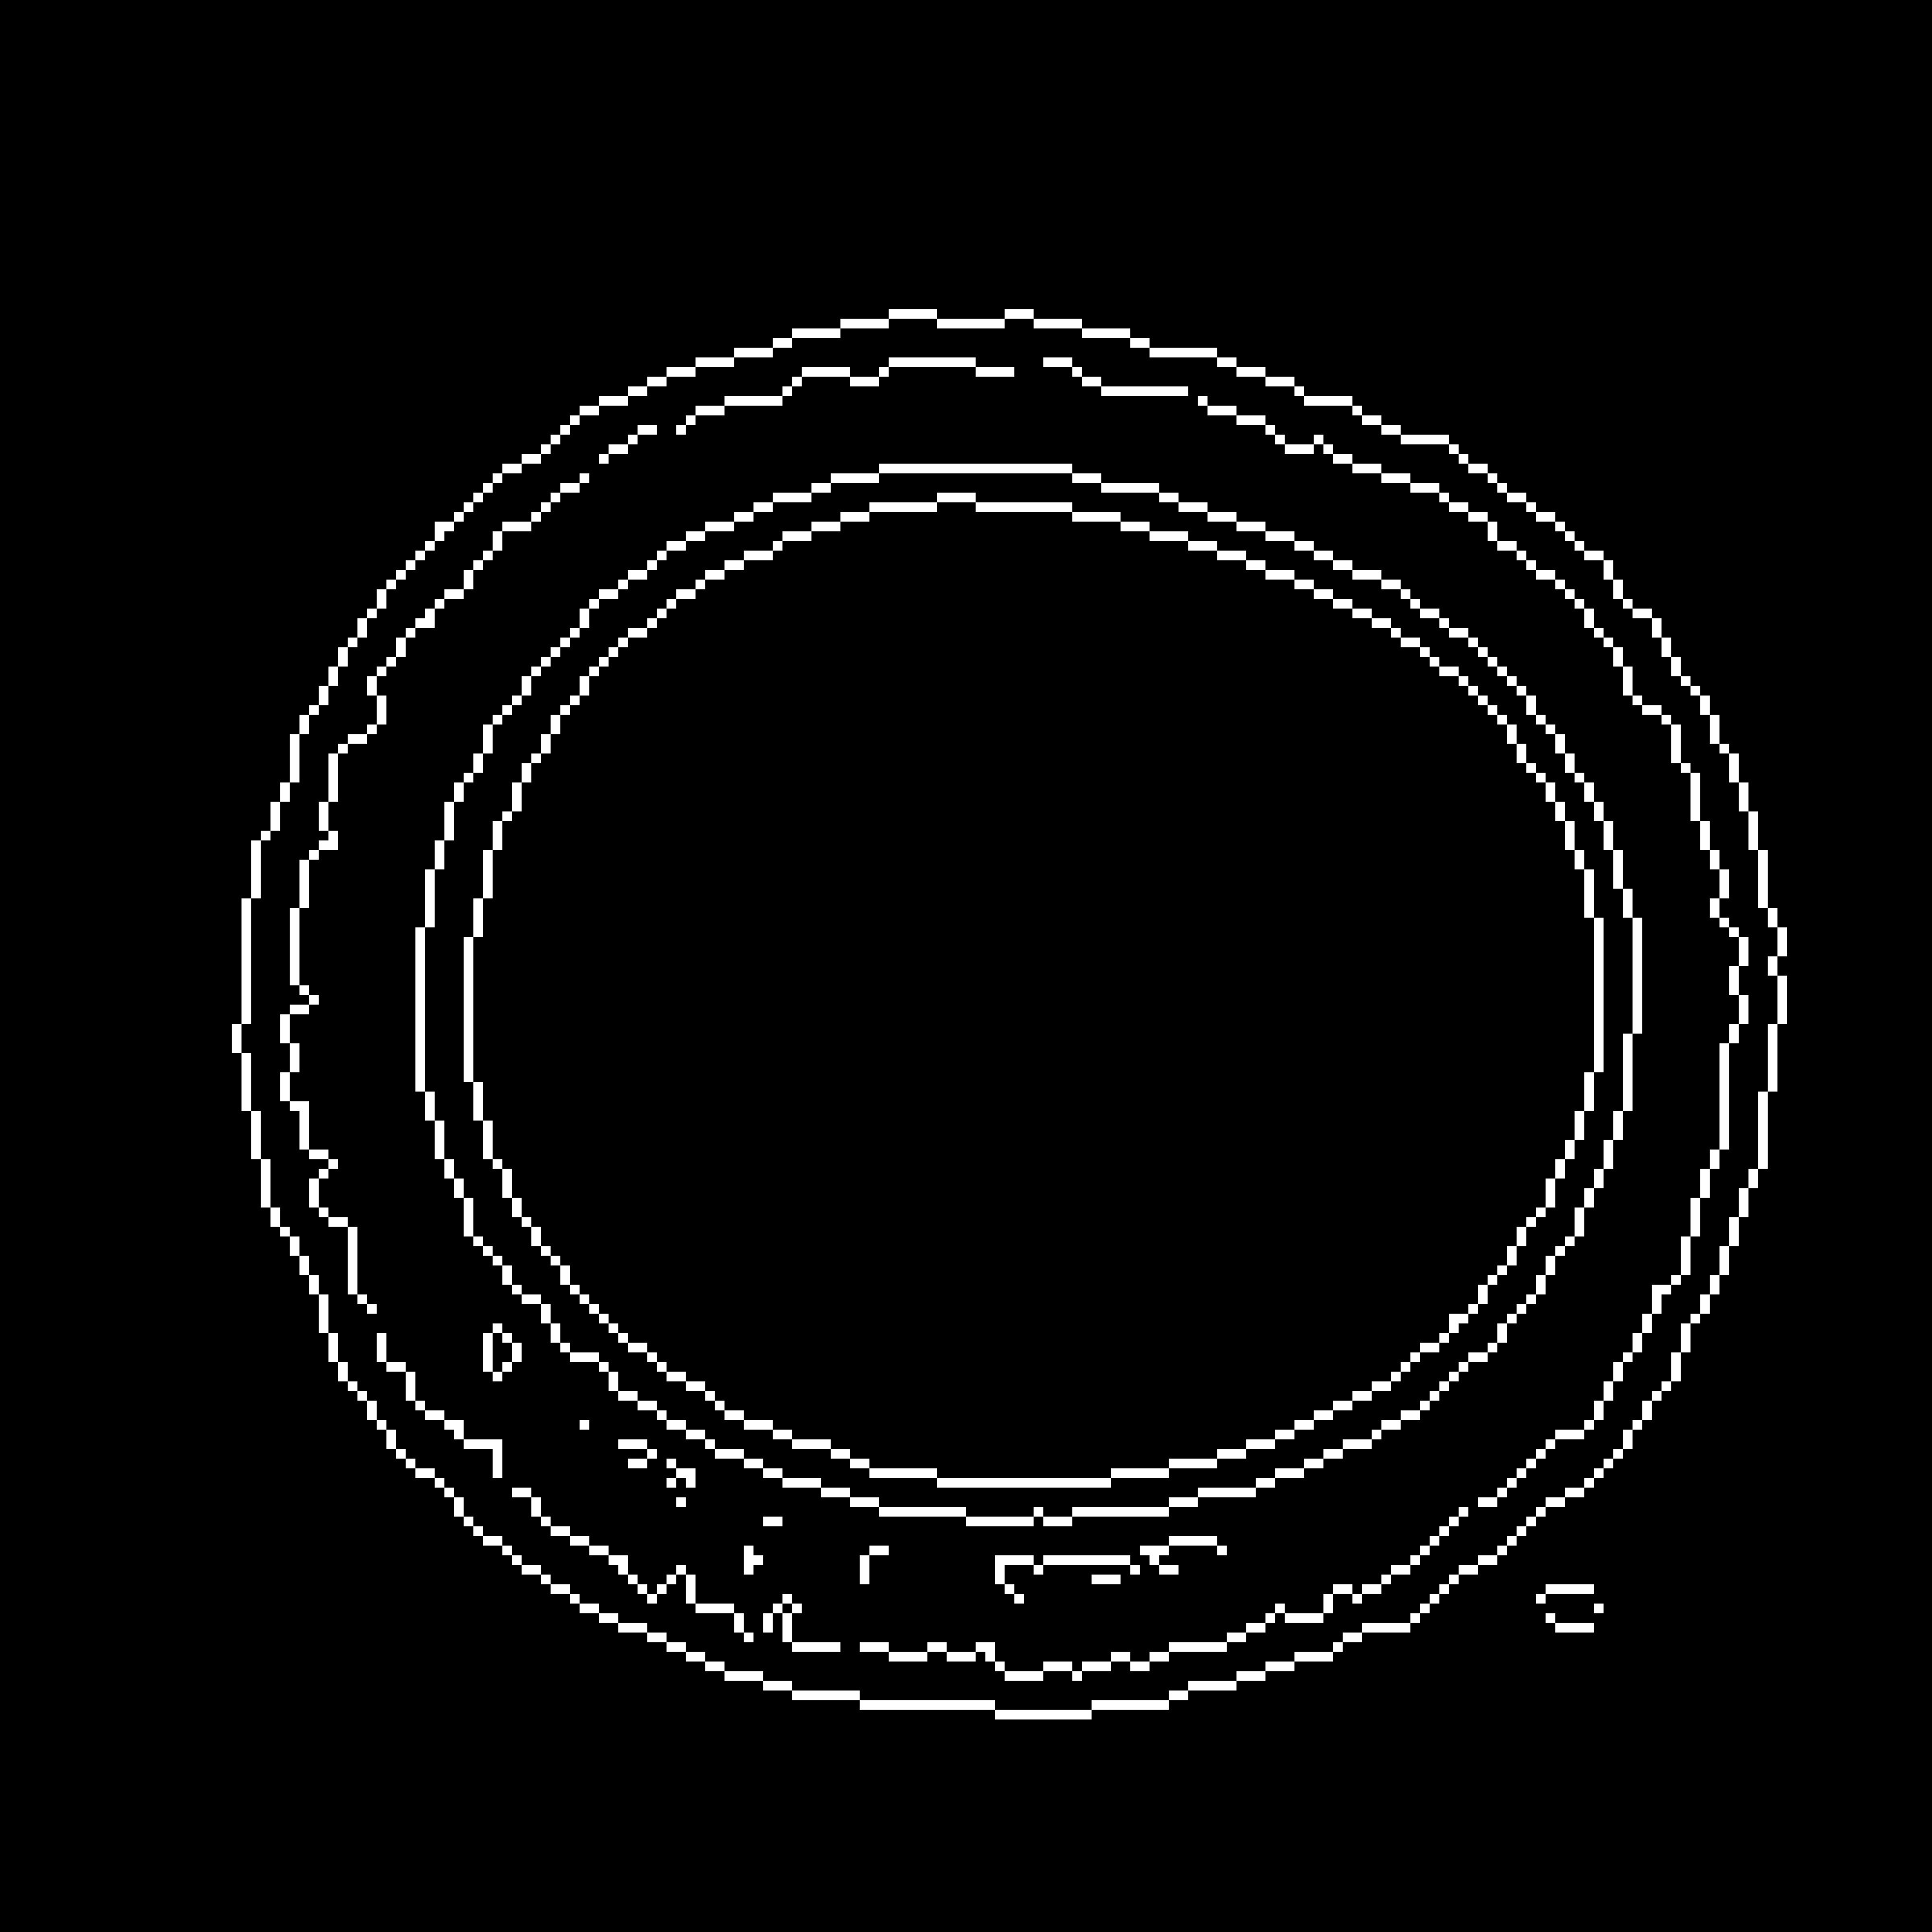
\includegraphics[width=0.1\textwidth]{membrane_scat_4}};					
    	\node[right=0.1in of fig4](fig5) {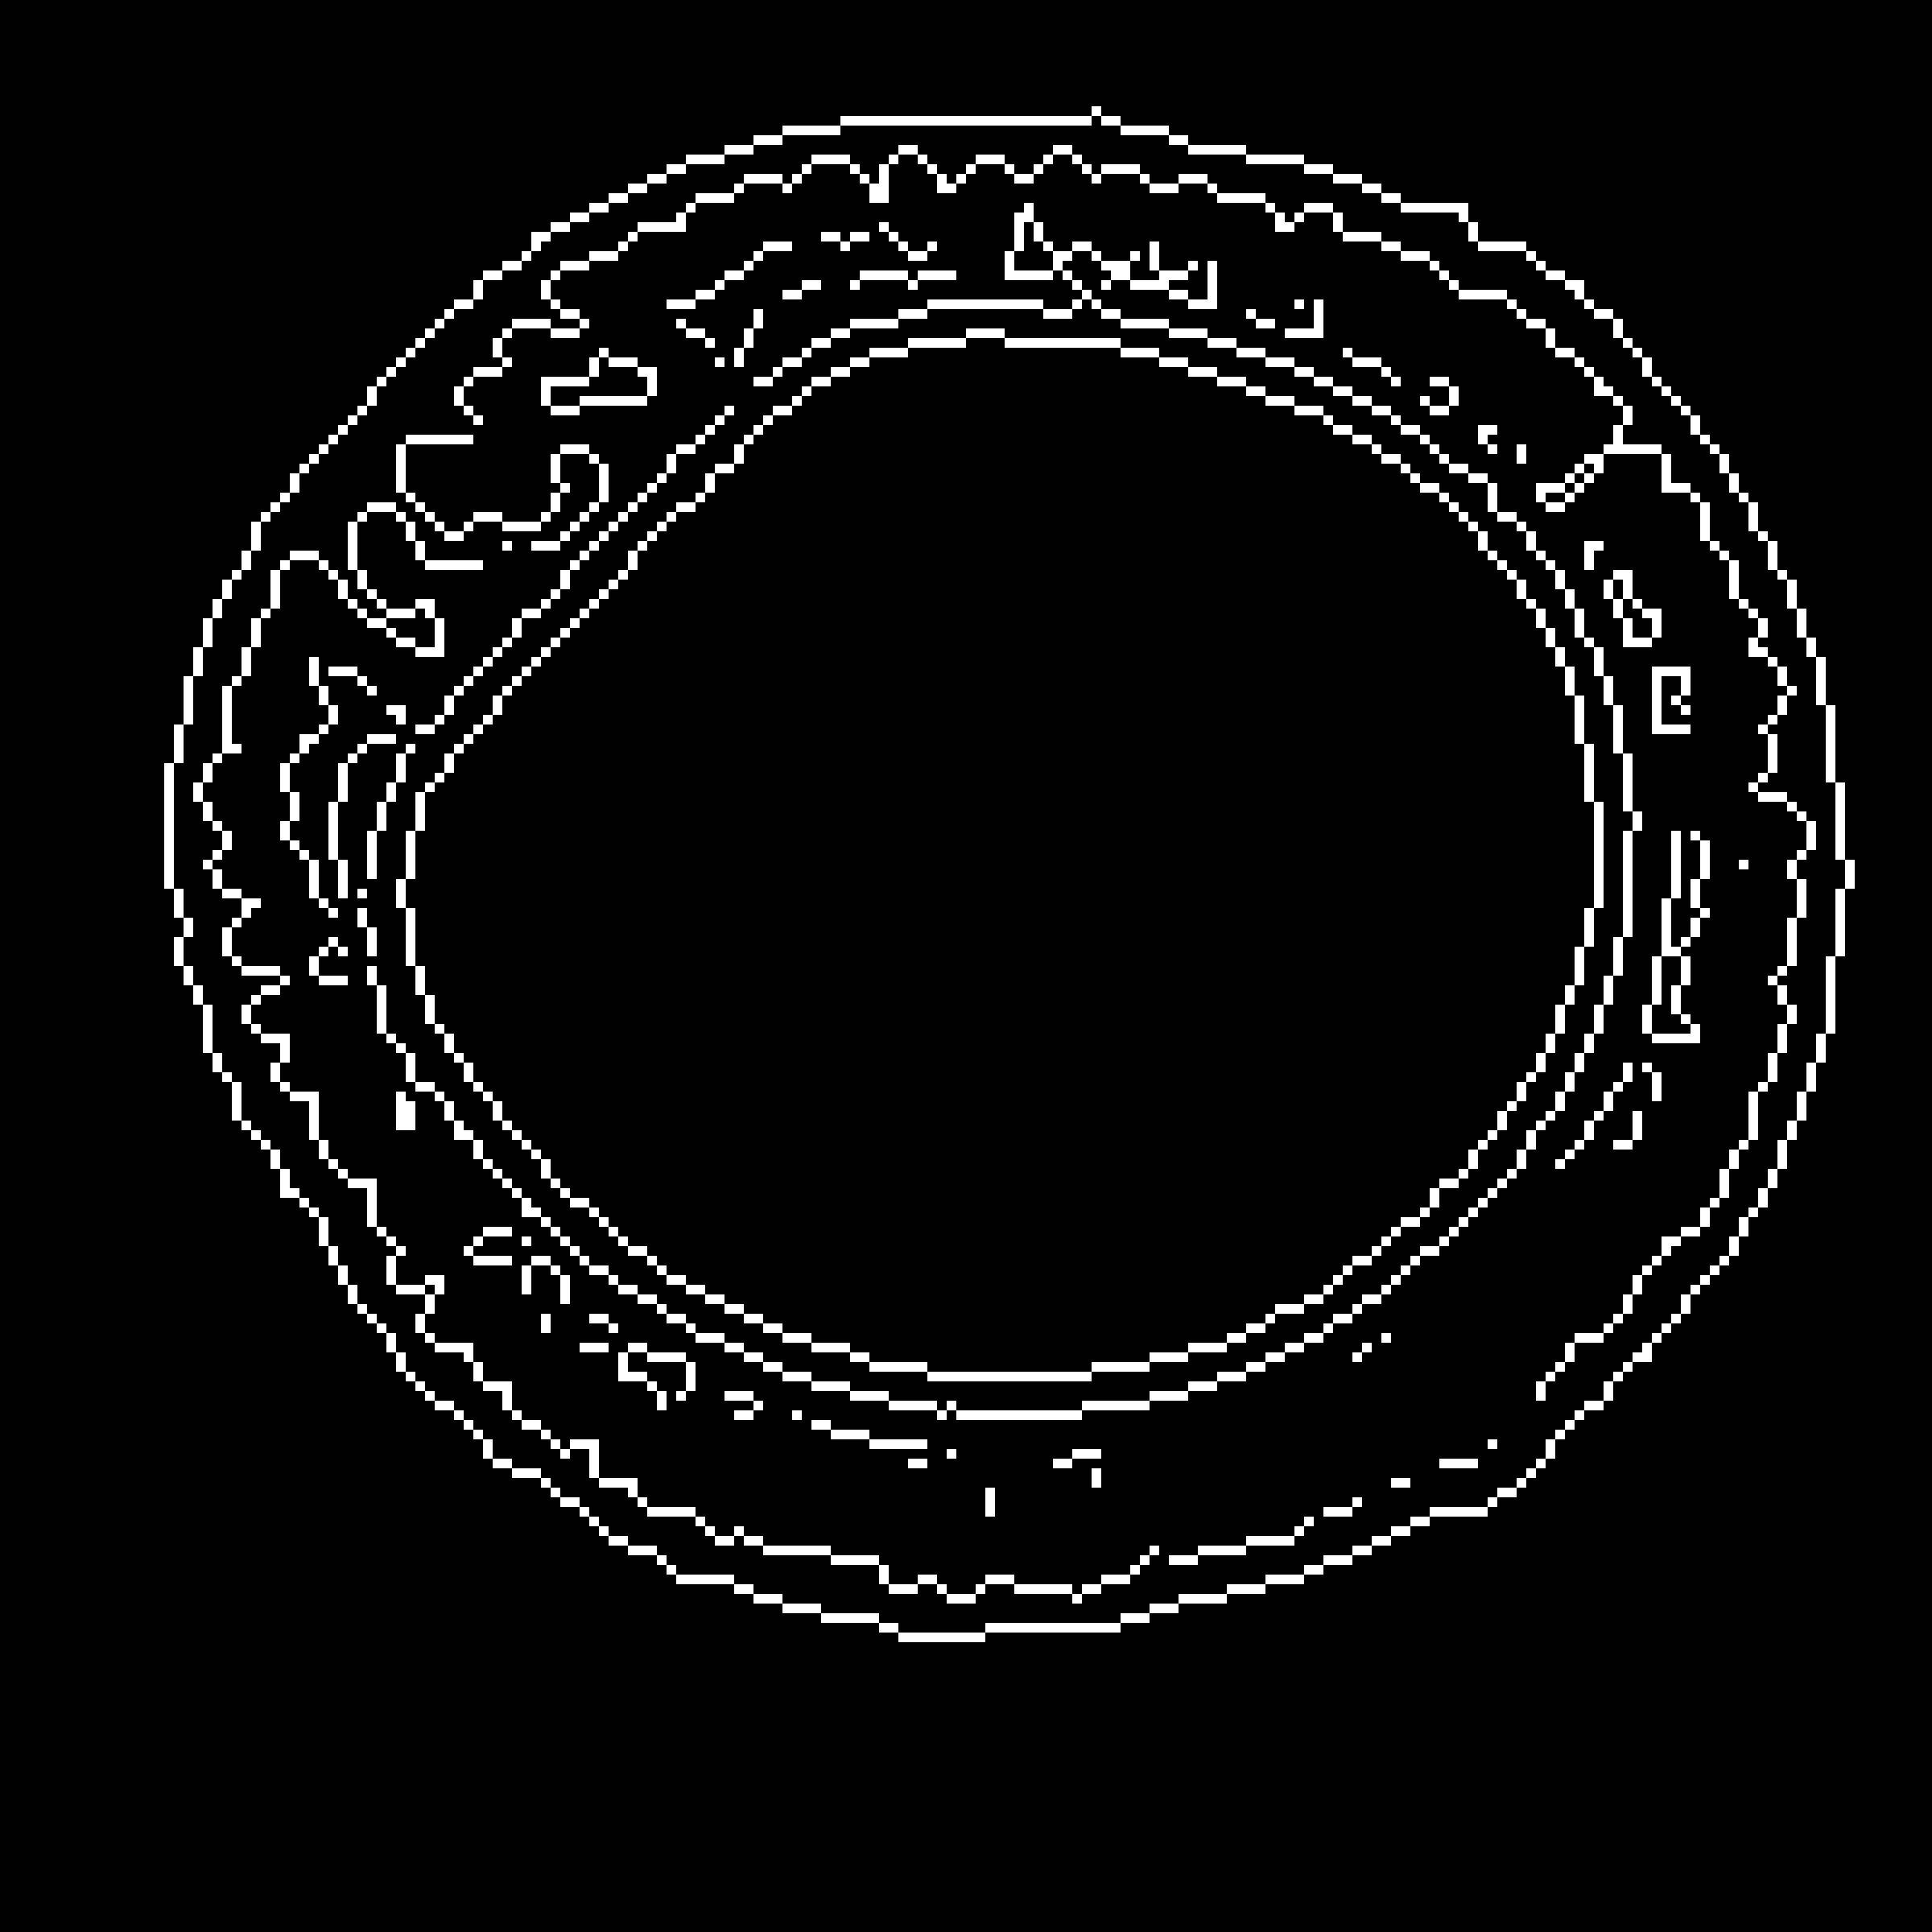
\includegraphics[width=0.1\textwidth]{membrane_scat_5}};
    	\node[below=0.02in of fig3](fig3b) {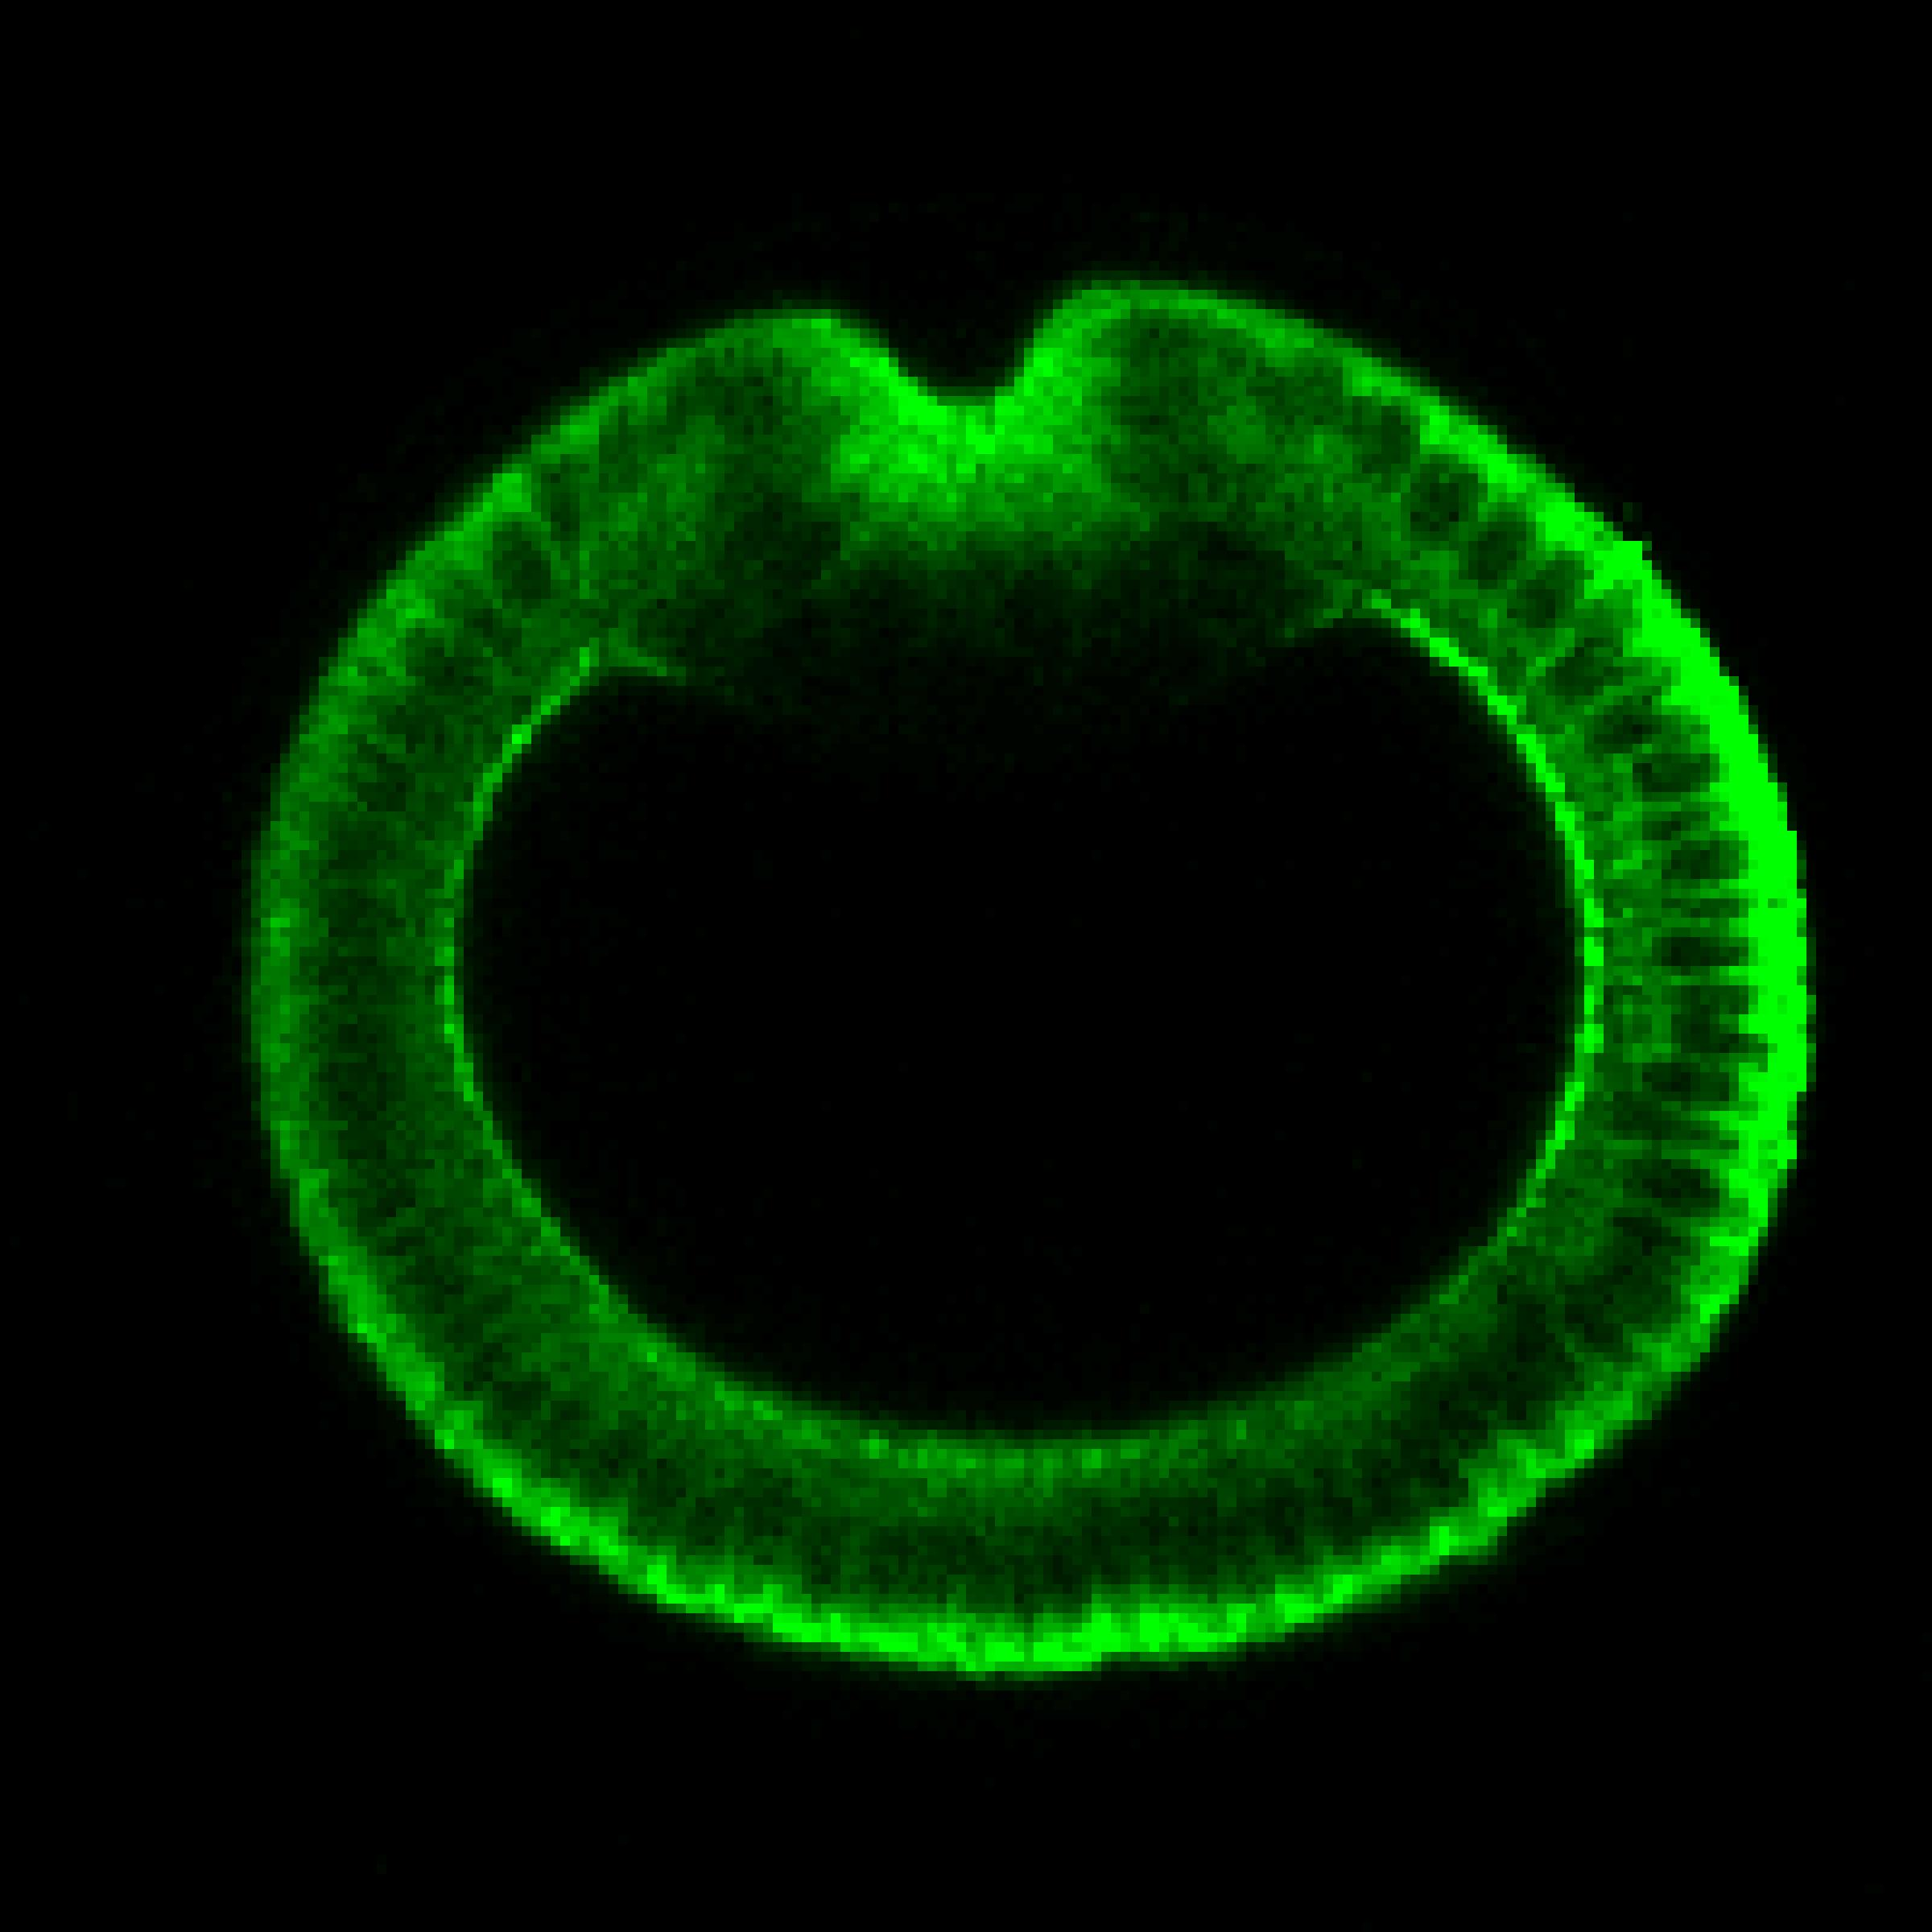
\includegraphics[width=0.1\textwidth]{membrane_scat_raw_3}};		
    	\node[left=0.1in of fig3b](fig2b) {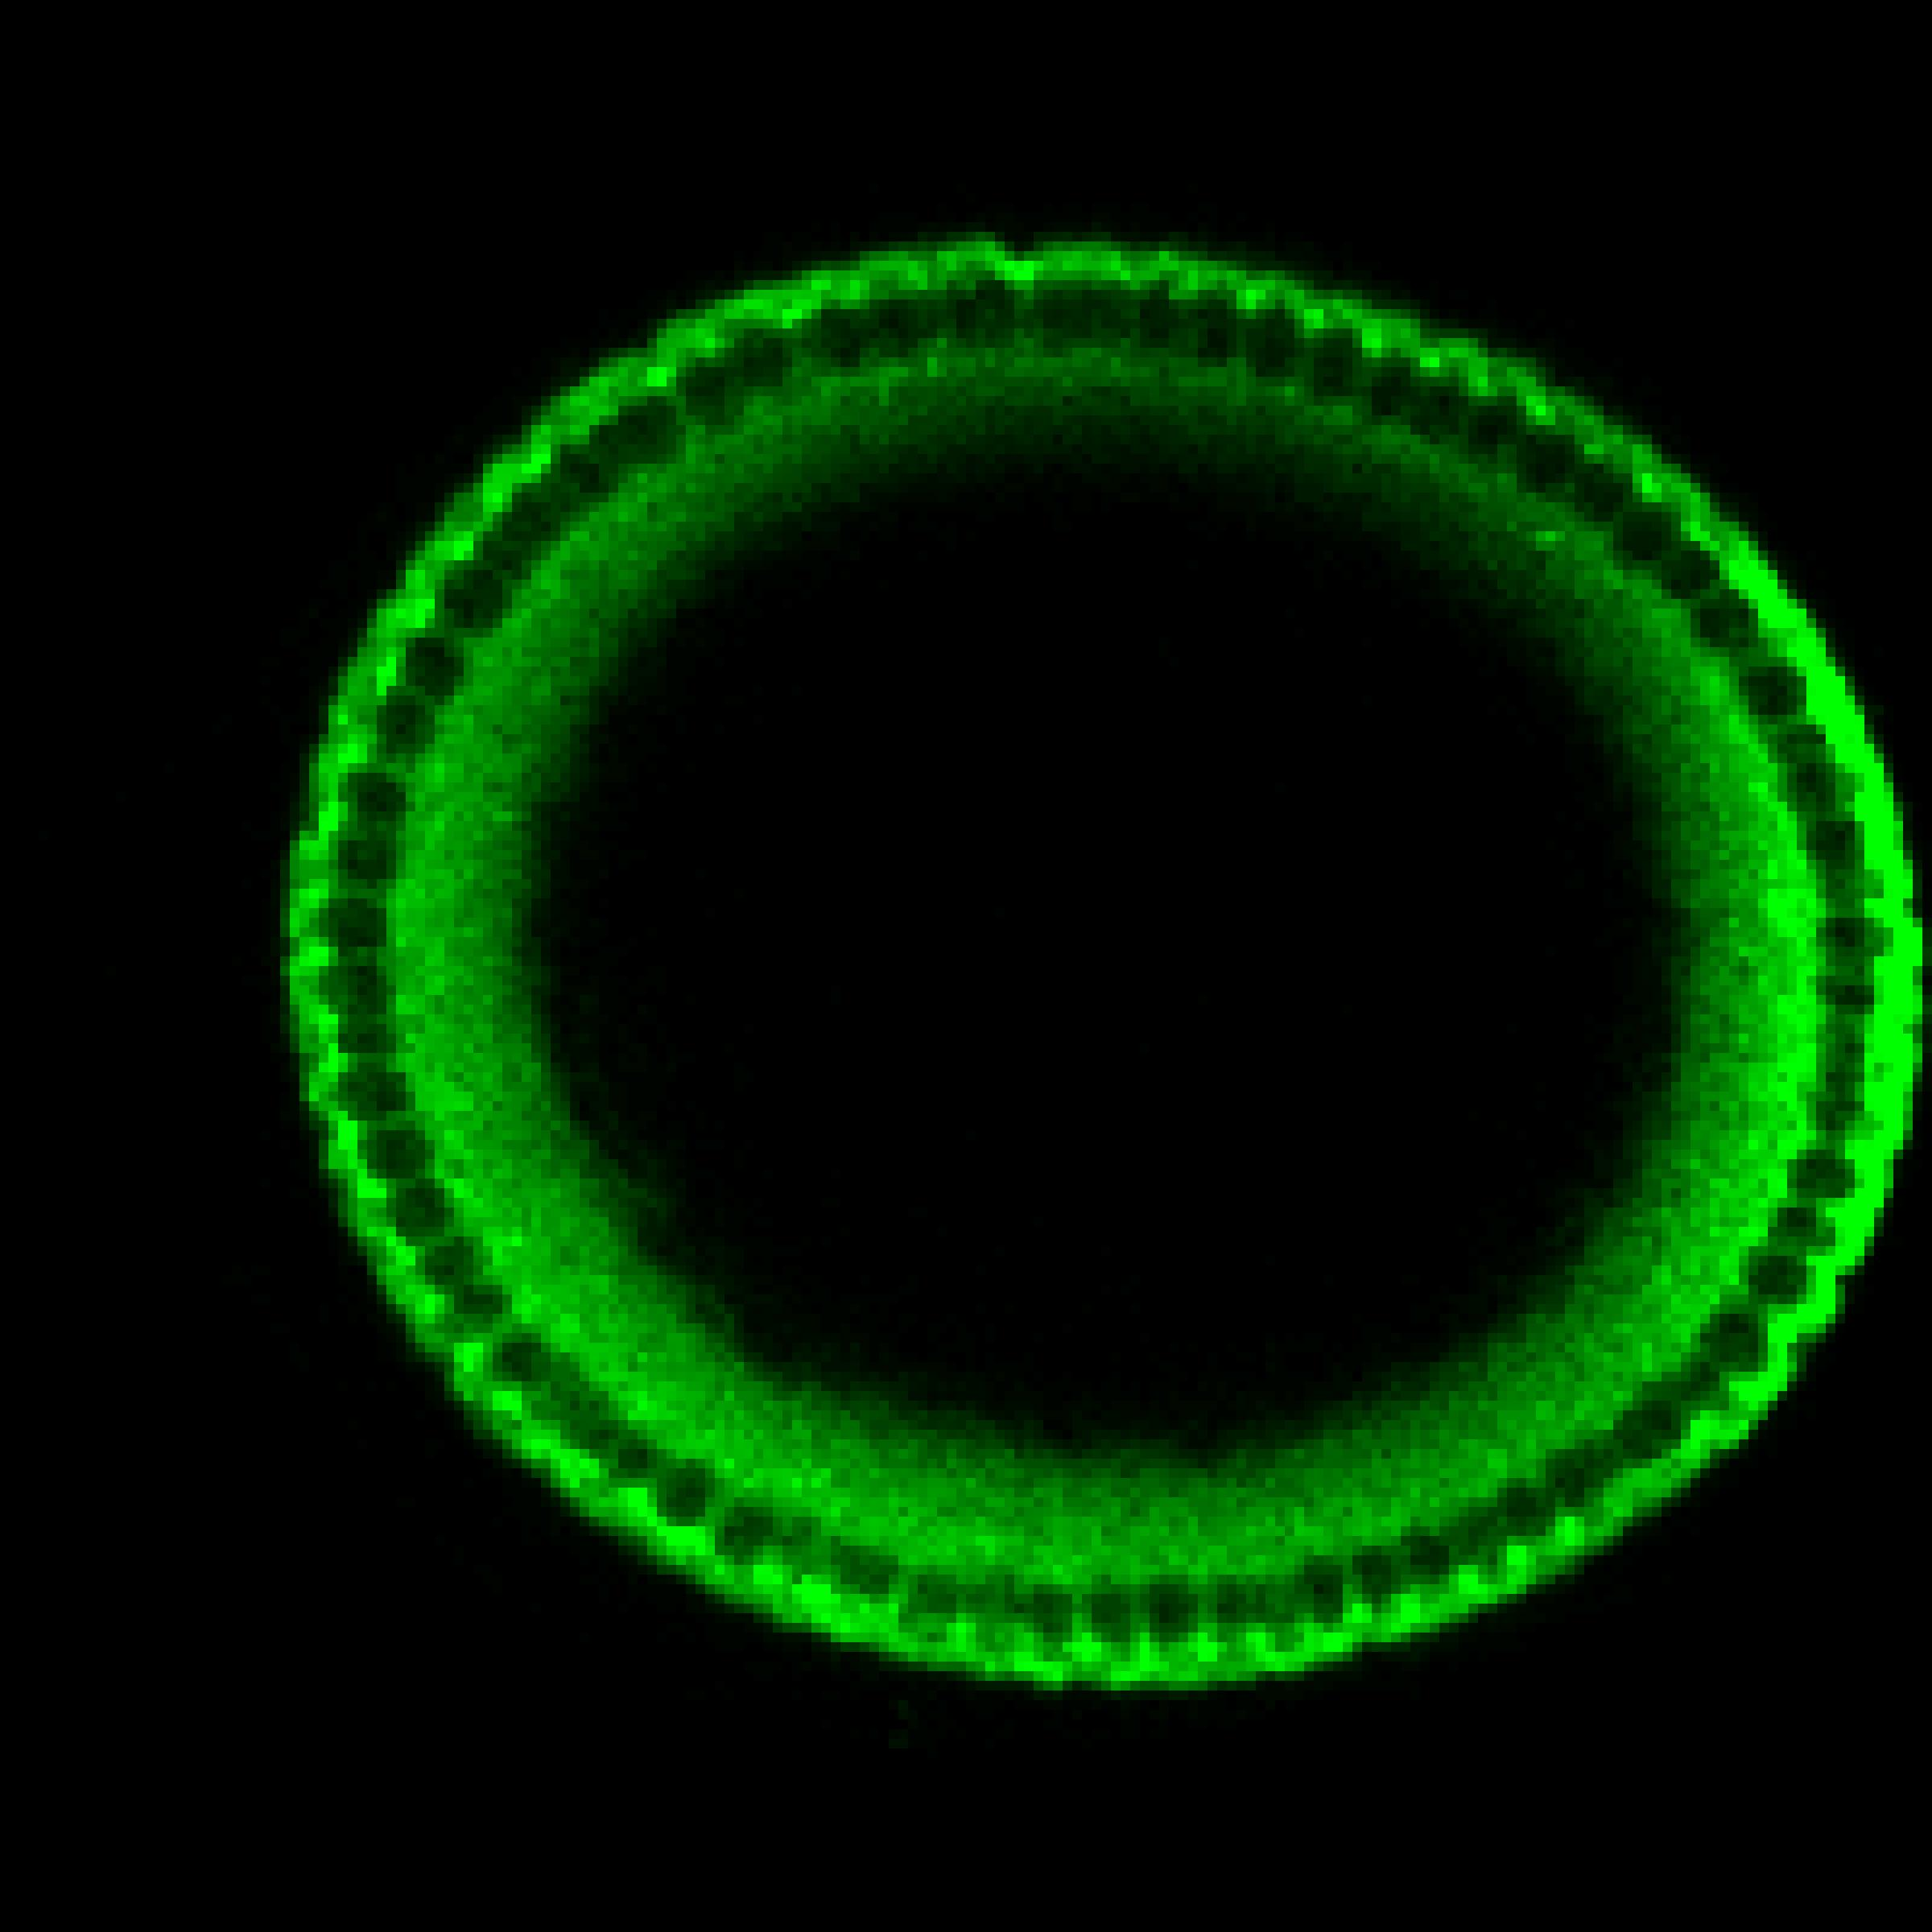
\includegraphics[width=0.1\textwidth]{membrane_scat_raw_2}};
    	\node[left=0.1in of fig2b](fig1b) {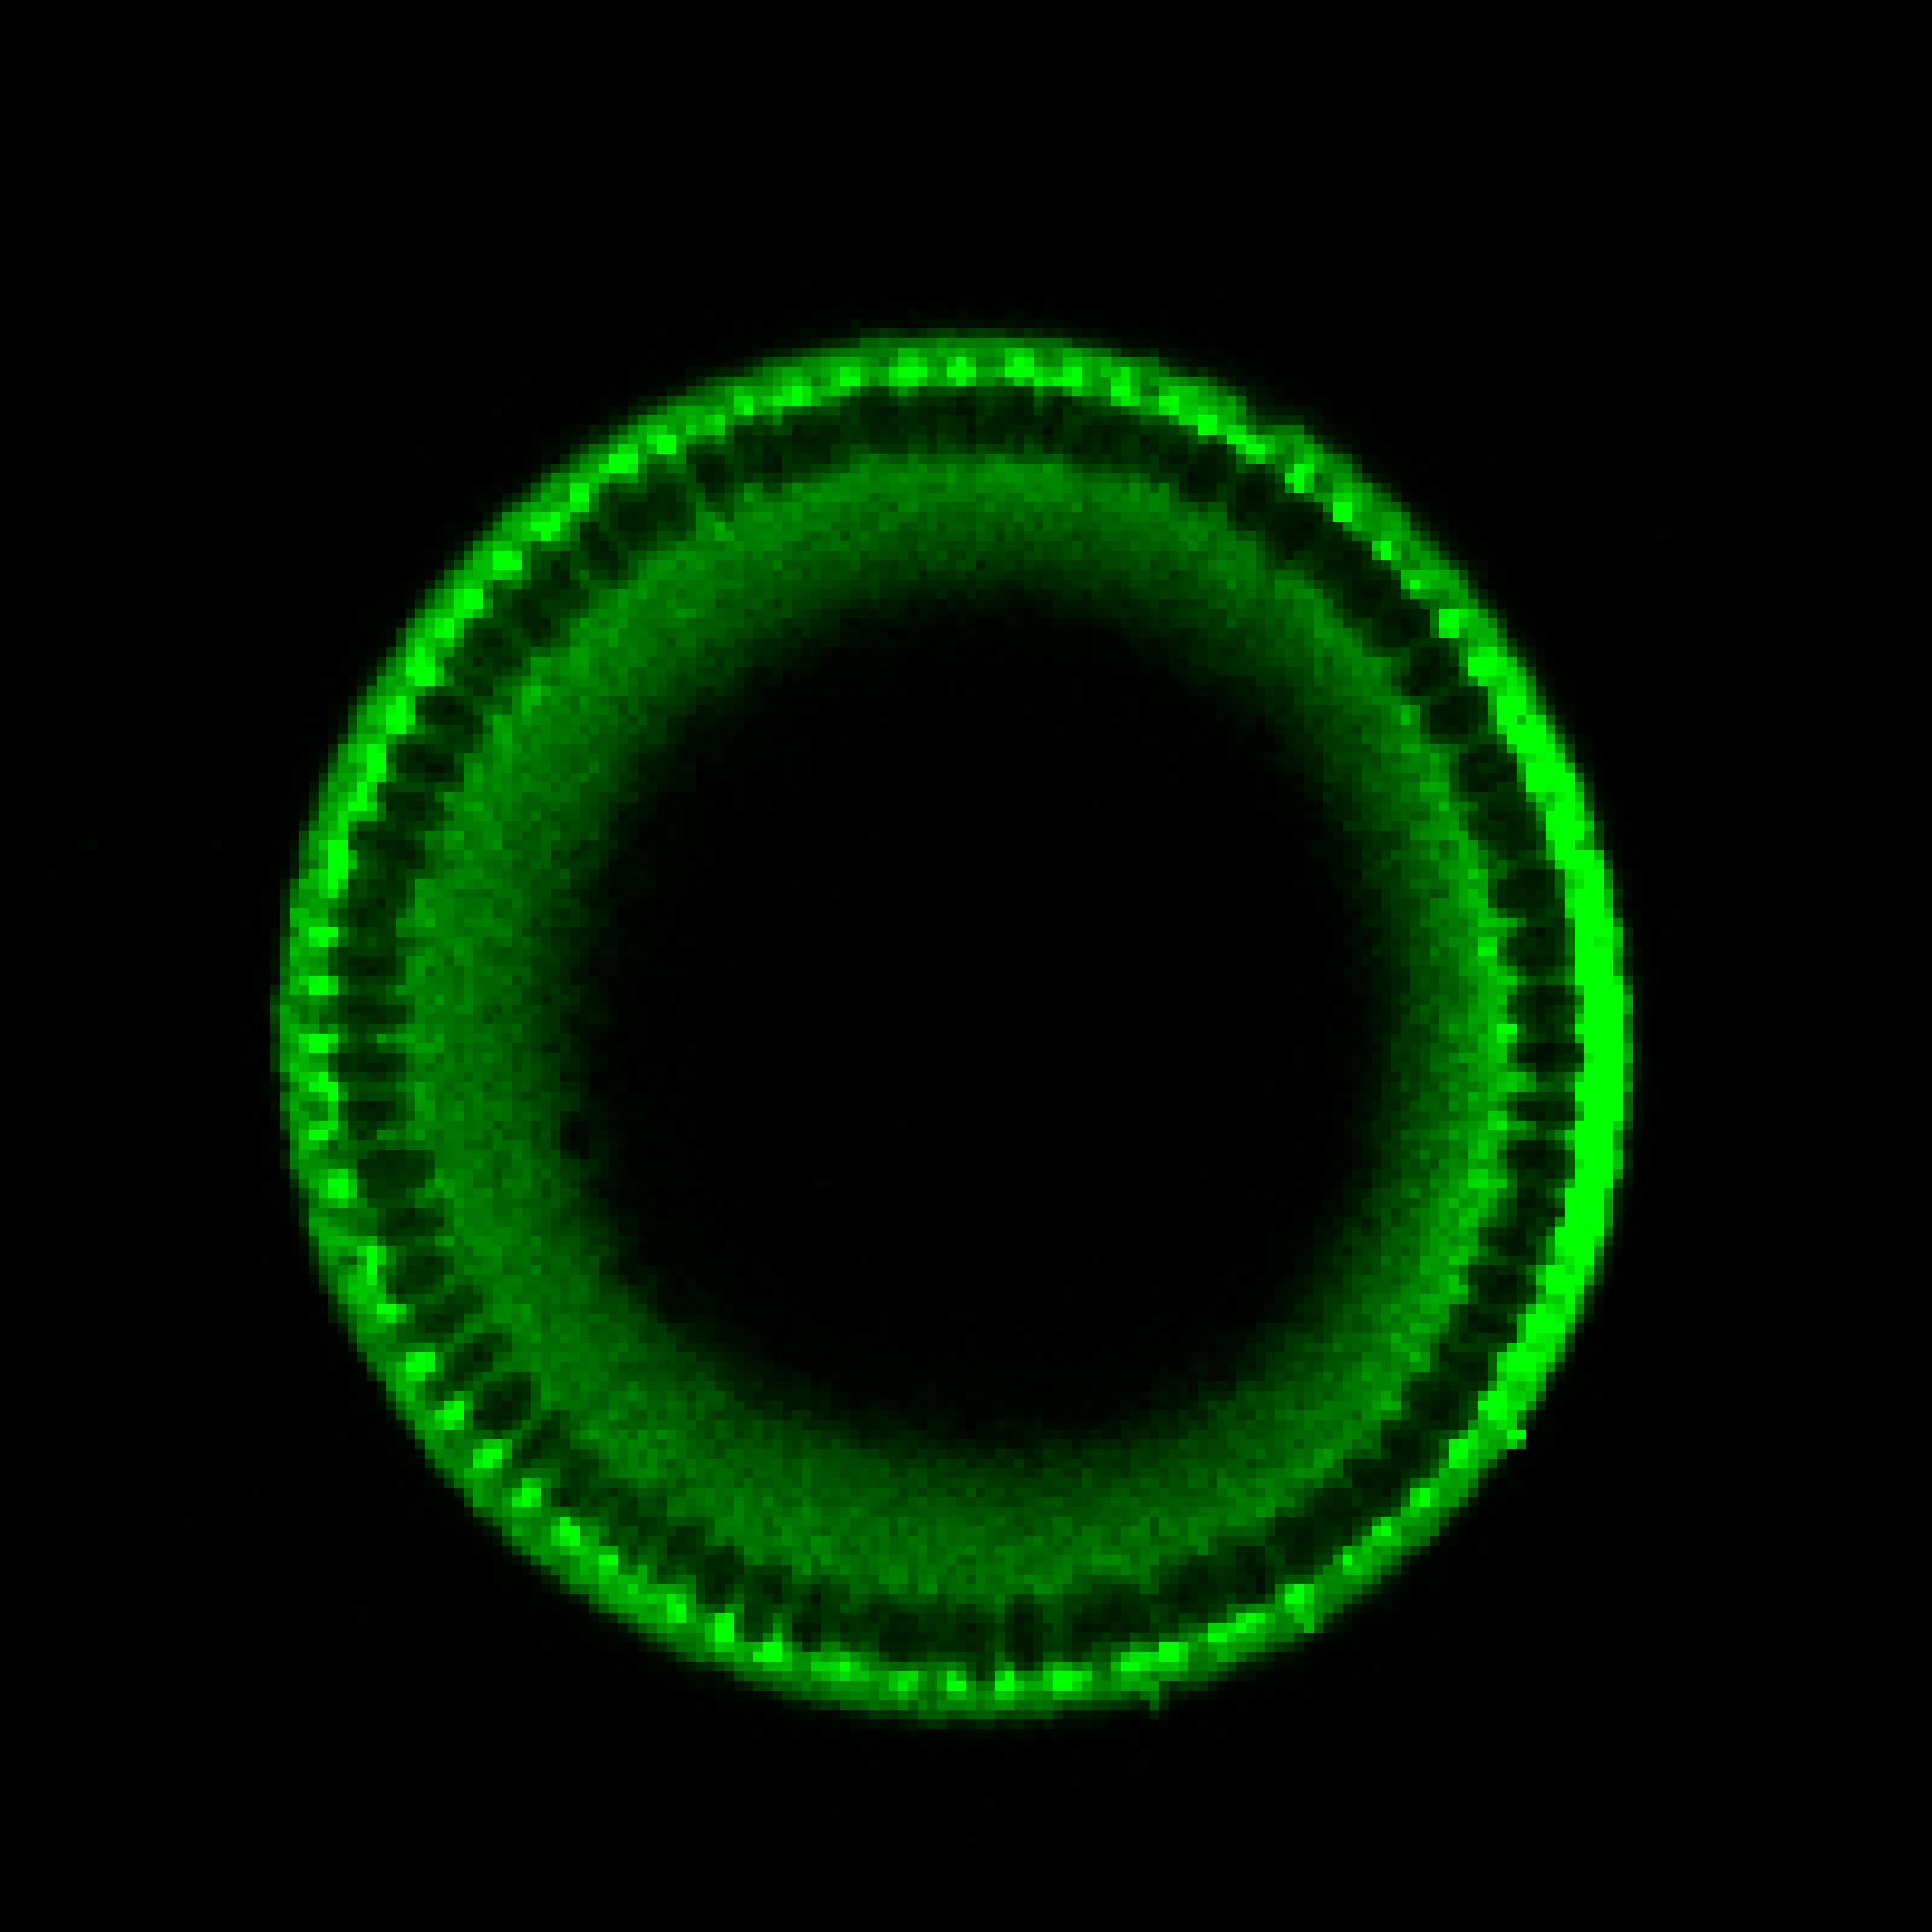
\includegraphics[width=0.1\textwidth]{membrane_scat_raw_1}};	
    	\node[right=0.1in of fig3b](fig4b) {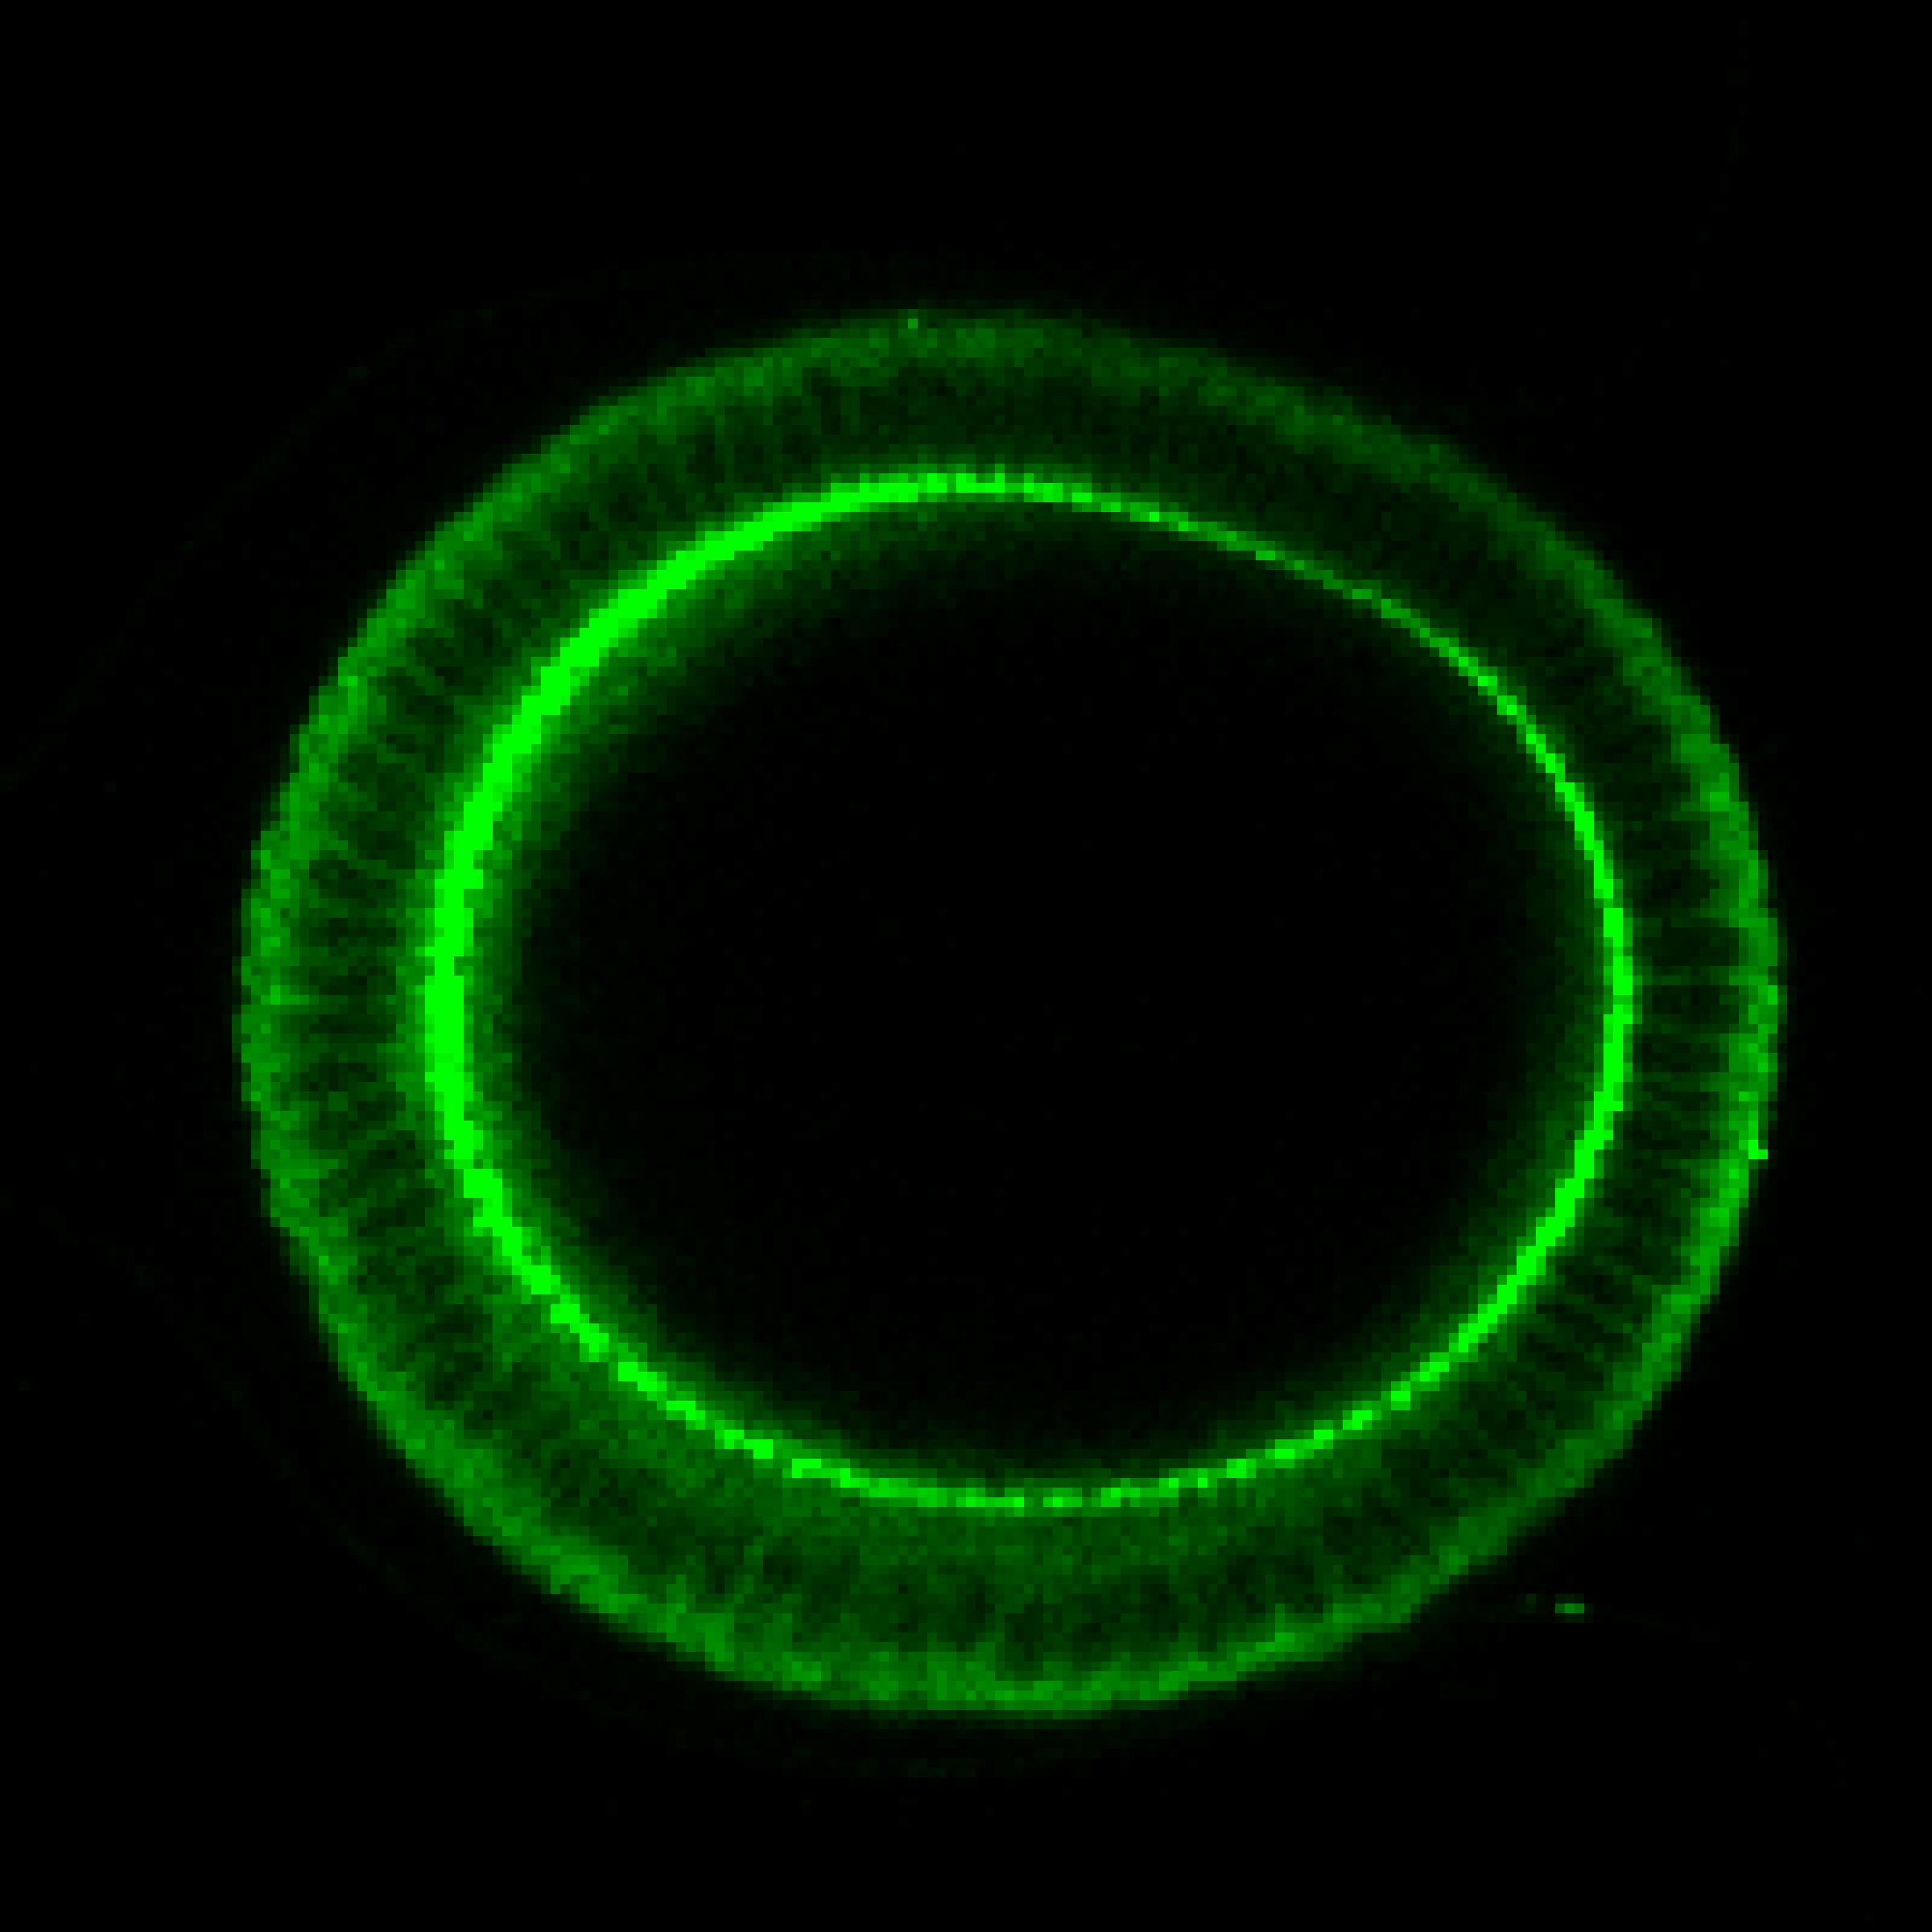
\includegraphics[width=0.1\textwidth]{membrane_scat_raw_4}};					
    	\node[right=0.1in of fig4b](fig5b) {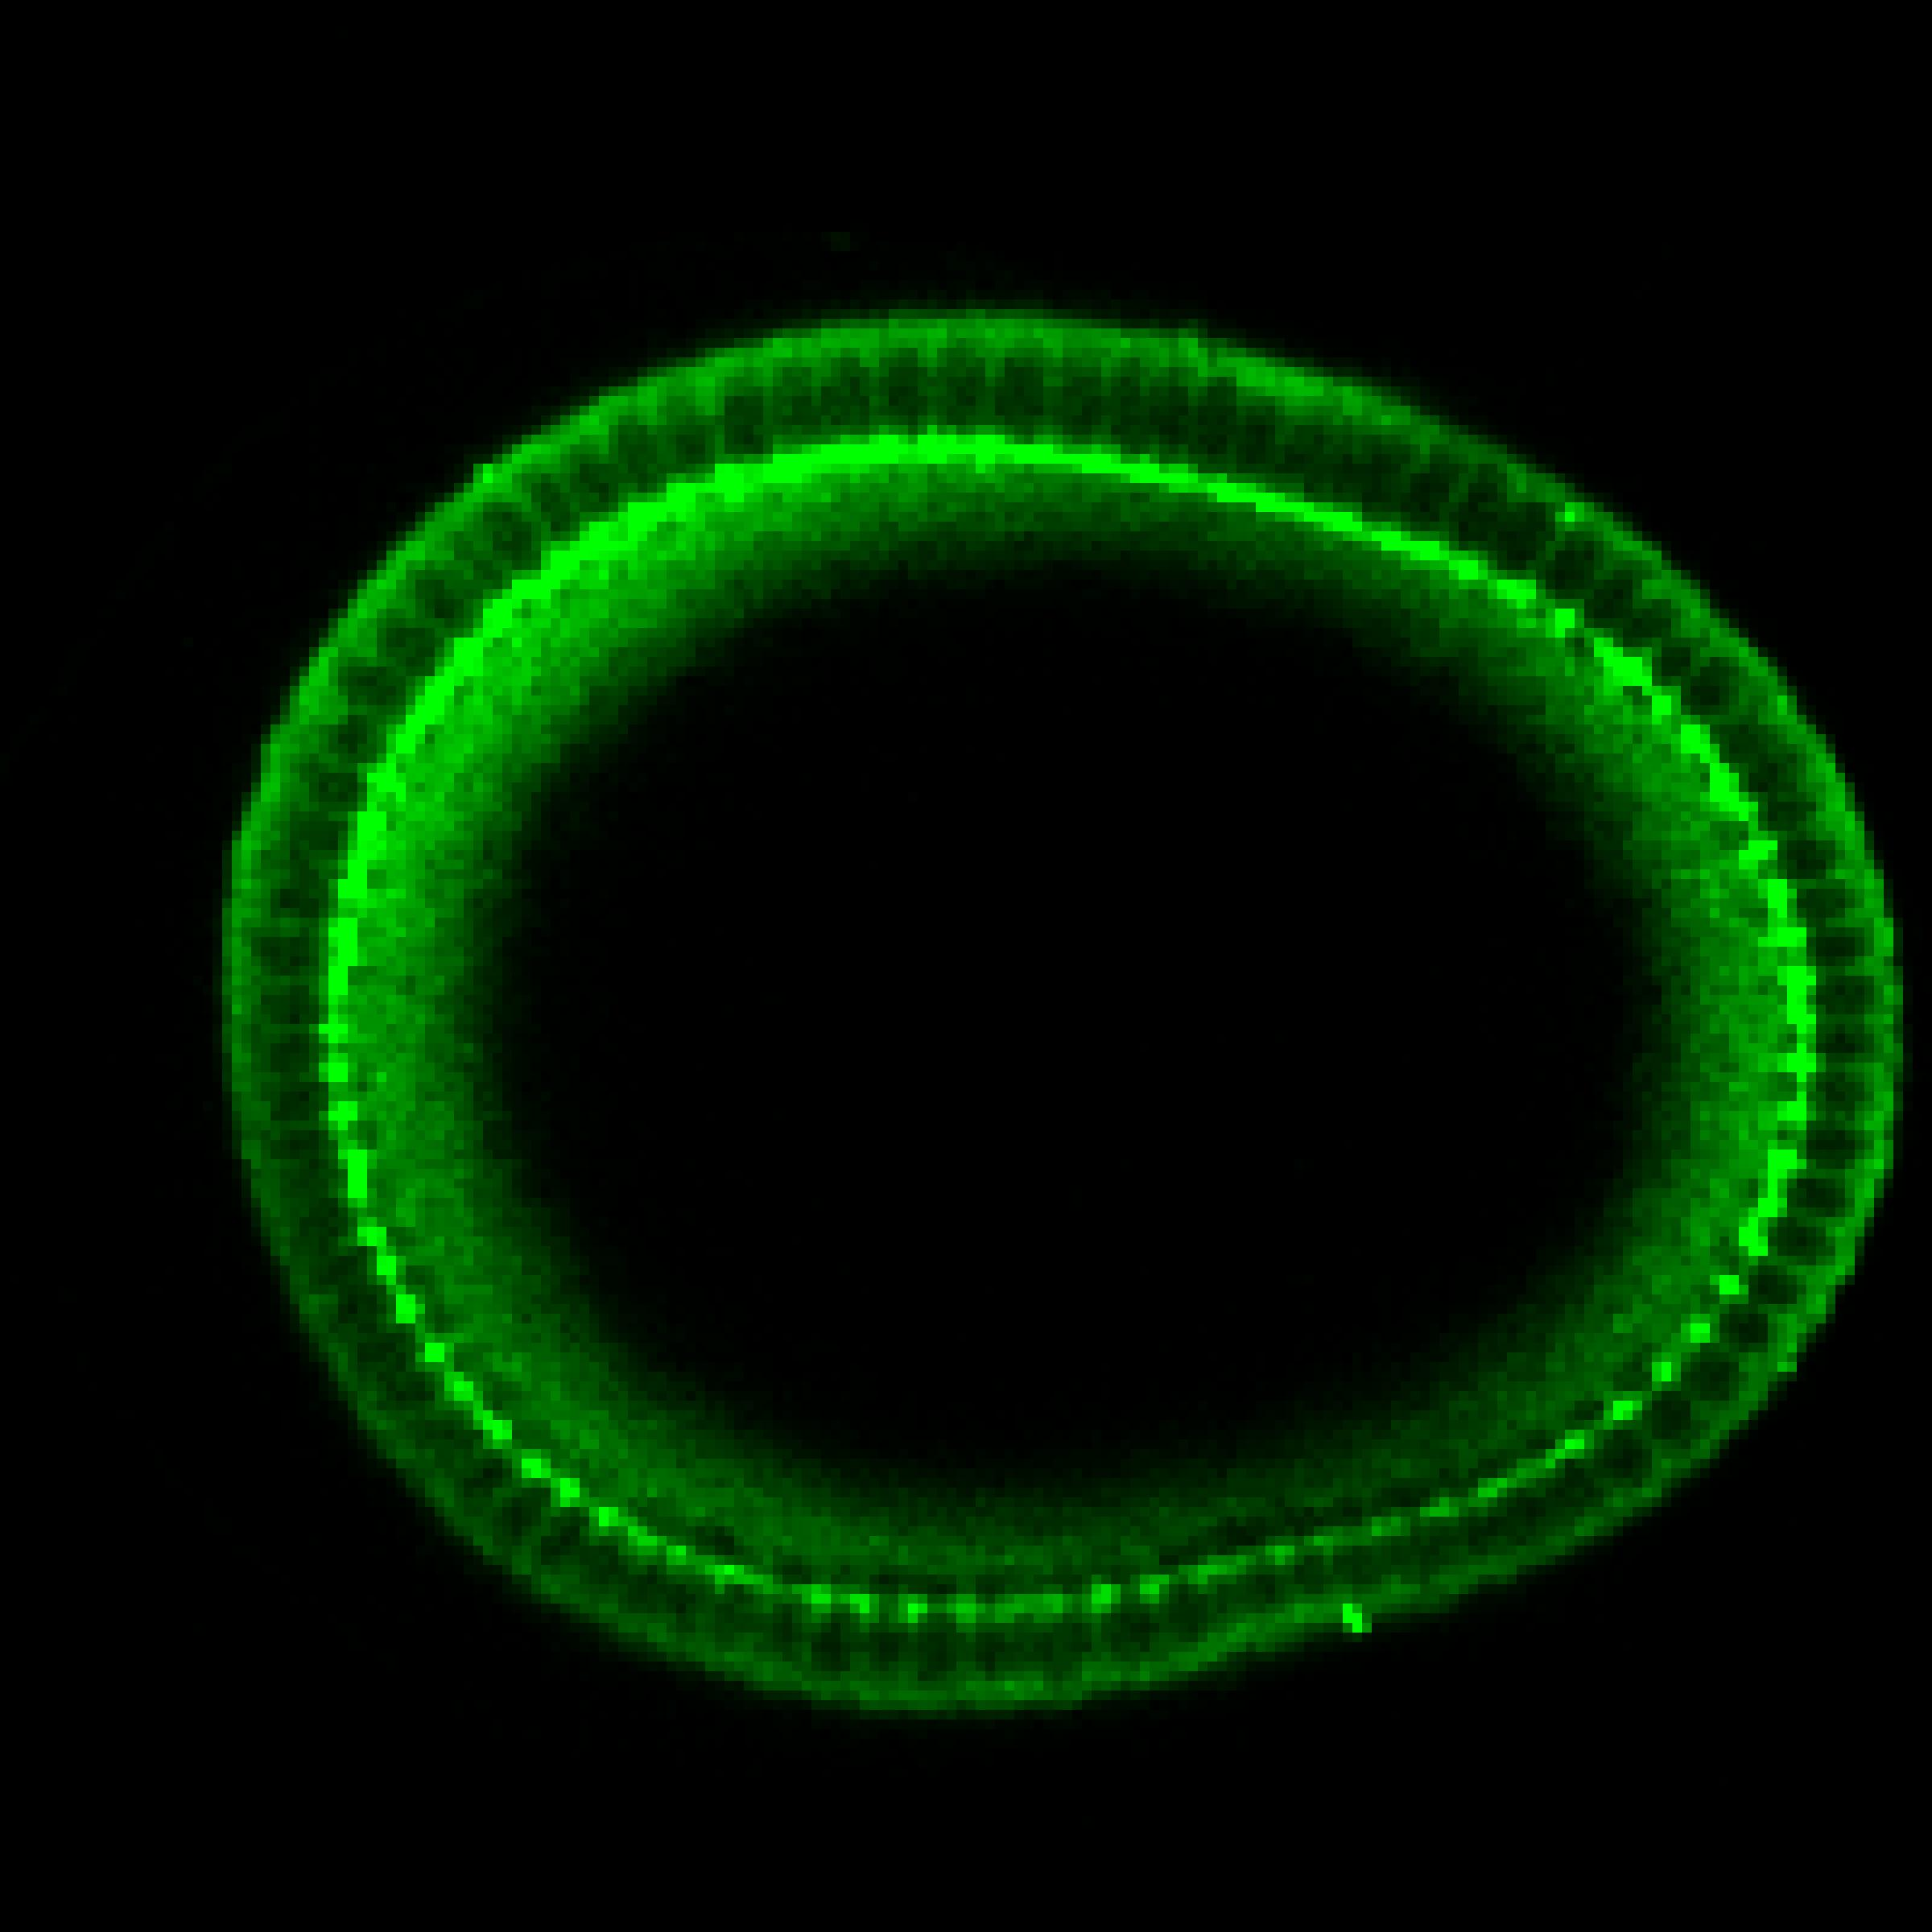
\includegraphics[width=0.1\textwidth]{membrane_scat_raw_5}};	    
    	\draw[->] (x1) -- (fig1.north);
    	\draw[->] (x2) -- (fig2.north);
    	\draw[->] (x3) -- (fig3.north);
    	\draw[->] (x4) -- (fig4.north);
    	\draw[->] (x5) -- (fig5.north);
    \end{tikzpicture}
    
\end{frame}

    
    

    